\documentclass[parskip=full, numbers=noenddot]{scrreprt}

\usepackage[english]{babel}
\usepackage[utf8]{inputenc}
\usepackage{csquotes}
%\usepackage[backend=biber, doi=false, isbn=false, url=false, date=year]{biblatex}
%\addbibresource{mainreport.bib}

% citations
\usepackage[
  natbib=true,
  backend=biber,
  doi=true,
  isbn=false,
  url=false,
  date=year,
  style=authoryear,
  citestyle=authoryear,
  minnames=1,
  maxnames=2,
  minbibnames=1,
  maxbibnames=99,
  uniquename=false,
  uniquelist=false]{biblatex}
\addbibresource{extendedreport.bib}
\usepackage{varioref}

\usepackage{graphicx}
  \graphicspath{ {./graphics/} }
\usepackage{url}
%\usepackage{varioref}
\usepackage{tabularx}
  \newcolumntype{L}{>{\raggedright\arraybackslash}X}
  \usepackage[version=4]{mhchem}
  \usepackage{siunitx}
  \usepackage{siunitx}
\DeclareSIUnit\molar{\mole\per\cubic\deci\metre}
\DeclareSIUnit\Molar{\textsc{m}}
\DeclareSIUnit\calorie{cal}
\usepackage{booktabs}
\usepackage{longtable}
\usepackage{ltablex}
\usepackage{pgfplotstable}
\usepackage{tikz}
\usetikzlibrary{shapes,arrows}
\usepackage{physics}

\author{Arin Wongprommoon\thanks{\texttt{arin.wongprommoon@ed.ac.uk, arin.wongprommoon@gmail.com}}
  \\University of Cambridge (Natural Sciences Tripos 2016-2019)
\\University of Edinburgh (PhD Candidate 2019 --)}
\title{Optimising production of citramalate based on \emph{E. coli} kinetic and stoichiometric models}
\subtitle{Extended project report}
\date{9 September 2019}

\begin{document}

\maketitle

\tableofcontents

\begin{abstract}

    Genetically modified \emph{E. coli} can be used to synthesise chemicals of industrial interest. For example, strains possessing citramalate synthase can produce citramalate ((2\emph{S})-2-hydroxy-2-methylbutanedioate), a precursor for the production of plastics.
  This project used modelling approaches to find conditions that maximise the production of citramalate. The kinetic model described by \citet{millard_metabolic_2017} and the stoichiometric model described by \citet{orth_comprehensive_2011}, both for \emph{E. coli} metabolism, were extended by adding a reaction that produced citramalate from acetyl coenzyme A and pyruvate.
  
  First, the effect of $V_{max}$ values of reactions in the kinetic model on productivity of citramalate was investigated. The differential evolution genetic algorithm was employed to compute the set of $V_{max}$ values of reactions that optimises the production of citramalate, assuming Michaelis-Menten kinetics. Differential evolution optimised $V_{max}$ combinations for ten reactions determined to have the greatest effects on citramalate productivity (CITRA\_SYN, GLT, LPD, GDH, ATP\_syn, ACEA, PYK, ZWF, NDHII, and MQO), and predicted the productivity of \num{405.5e-4} h\textsuperscript{-1}.

  In the second part of the project, information from the kinetic model was used in the kinetic model to enrich the stoichiometric model. The possible values of fluxes through each reaction were used to set the bounds for each reaction in the stoichiometric model. A strategy of mapping reactions between the kinetic model and the stoichiometric model was devised. Flux balance analysis (FBA) was then performed to evaluate the highest possible flux through the citramalate synthesis reaction as a proxy for citramalate productivity. This achieved an optimum solution of 0.2922 mM s\textsuperscript{-1}, and subsequent analysis of flux bounds saw concordance with what is expected \emph{in vivo}. Finally, composition of the Lund medium \citep{eastham_process_2015} was studied in an attempt to create bounds for relevant uptake reactions.
  
\end{abstract}

\chapter*{Introduction}
\label{ch:intro}

Using living organisms to synthesise chemicals is an alternative to synthesising chemicals from fossil fuels, as it serves as a renewable resource with potentially high efficiency and low costs. The procedures can be sped up by using mathematical models to optimise conditions. Citramalate ((2\emph{S})-2-hydroxy-2-methylbutanedioate) is a chemical of industrial interest as it can be a precursor for methacrylic acid, a monomer for the production of plastics. \emph{E. coli} was chosen as the model organism because its metabolism is well-characterised in mathematical models, because predictions from models can be verified in cultures that are easy to maintain, and because there are \emph{E. coli} strains that have been genetically engineered to produce citramalate.

Citramalate synthesis is mediated by citramalate synthase (EC 2.3.1.182) in \emph{Methanococcus janaschii} \citep{wu_production_2016}, which catalyses the reaction:

\begin{center}
  acetyl-CoA + pyruvate + \ce{H2O} $\rightarrow$ CoA-SH + \ce{H^+} + citramalate
\end{center}

This enzyme is not present in wild-type \emph{E. coli} strains, so in experiments \emph{E. coli} is engineered to express the \emph{cimA} gene that encodes citramalate synthase \citep{wu_production_2016}.

This project concerns two models of \emph{E. coli} metabolism: a kinetic model described by \citet{millard_metabolic_2017} and a stoichiometric model described by \citet{orth_comprehensive_2011}.
The stoichiometric model is a genome-scale reconstruction of the \emph{E. coli} metabolic network. In contrast, the kinetic model only concerns central carbon metabolism, but contains initial conditions and substrate concentrations, which the stoichiometric model lacks.

This project had the following aims:

\begin{enumerate}
\item Investigating how $V_{max}$ values of reactions in the kinetic model affect citramalate productivity, and finding a method to find such values that would optimise citramalate productivity;
\item Enriching the stoichiometric model with information from the kinetic model regarding fluxes through reactions, along with reconciling differences between the models in mapping reactions; and
  \item Using information from the Lund medium \citep{eastham_process_2015} on the models to determine how nutrient medium composition affects citramalate productivity, and investigating how this information can be used to improve the Lund medium.
\end{enumerate}

The kinetic model contains 68 reactions, 49 of which include $V_{max}$ as a parameter (see appendix~\ref{ap:kineticreactionlist}). Of these, 41 correspond to real enzyme-catalysed reactions.
To investigate citramalate production, a 69th reaction called CITRA\_SYN was added to the kinetic model to model citramalate synthesis.  In the model, this reaction has the Michaelis-Menten kinetic law:

\begin{equation}
  \frac{\mathrm{d}[citramalate]}{\mathrm{d}t} = 
  \frac{V_{max} \cdot [acetyl-CoA]}{[acetyl-CoA] + K_{m}}
\end{equation}
\label{eq:michaelismenten}

This kinetic law assumes that pyruvate is saturating. $V_{max}$ is set to 4 mM s\textsuperscript{-1} and $K_{m}$ to 0.495 mM in the modified model. These values are based on experimental values obtained in the ConBioChem project.

Manipulating the SBML file encoding the kinetic model required the Python library \texttt{libsbml} \citep{bornstein_libsbml:_2008} and running simulations employed the \texttt{roadrunner} \citep{somogyi_libroadrunner:_2015} module. The simulations ran from 0 to 7,200 seconds, at which steady-state was attained for almost all conditions.
Using this modified kinetic model, I investigated the effect of parameters on citramalate productivity. Citramalate productivity is defined as $\mu \cdot Y_{P/S}$, where $\mu$ is the growth rate in reciprocal time units (h\textsuperscript{-1}) and $Y_{P/S}$ is defined as the mass of the product (citramalate) divided by the mass of the substrate (glucose).


The stoichiometric model contains 2,584 reactions, and I mapped 57 to their equivalents in the kinetic model. By default, most of these reactions are unbounded \citep{orth_comprehensive_2011}.
A 2,585th reaction for citramalate production was added to the stoichiometric model using the \texttt{cobra} module \citep{ebrahim_cobrapy:_2013} in Python. This reaction contains the same information as the reaction added to the kinetic model except for the kinetic law, which is normally absent from stoichiometric models. In addition, a sink reaction to allow citramalate to leave the system was also added.
Fluxes through reactions in the stoichiometric model were investigated using flux balance analysis, or FBA \citep{orth_what_2010}, and FBA simulations employed the \texttt{cobra} module.

% [This might be more appropriate in the discussion; it is an important part of the project and it does relate the two models, but it seems out of place in an otherwise `expository' introduction. If this is moved to the discussion, I might comment on using different values for the ratio between cell dry weight and cell volume, but I honestly don't think it's important enough to deserve a mention]
The kinetic and stoichiometric models use different units. Fluxes are in mM s\textsuperscript{-1} in the kinetic model, but are mmol g\textsubscript{DW}\textsuperscript{-1} h\textsuperscript{-1} in the stoichiometric model. Using the cell volume of \num{1.77e-3} L g\textsubscript{DW}\textsuperscript{-1} as specified in the kinetic model, I worked out that converting values from the kinetic model to the stoichiometric model involves multiplying by 6.372\footnote{
($R$ mM s\textsuperscript{-1})(\num{1.77e-3} L g\textsubscript{DW}\textsuperscript{-1})(3600 s h\textsuperscript{-1}) = 6.372 $R$ mmol g\textsubscript{DW}\textsuperscript{-1} h\textsuperscript{-1}
}.
Because the stoichiometric model does not have information about enzyme kinetics, the values associated with the kinetic model (with kinetic model units) can be used with the structure of the stoichiometric model without any adjustments.

\chapter{Investigating the kinetic model}
\label{ch:kinetic}

I investigated the kinetic model to determine the combination of $V_{max}$ values that would optimise citramalate productivity. This parameter was chosen as it can be easily tested \emph{in vivo} by relying on the principle that $V_{max}$ is proportional to enzyme concentration. I started from varying $V_{max}$ values one and two reactions at a time to establish patterns. Then, I used differential evolution to vary multiple $V_{max}$ values simultaneously, employing the genetic algorithm to narrow down the solution space.

\section{Varying $V_{max}$ values one reaction at a time}
\label{sec:onereac}

The kinetic model includes 49 reactions that have $V_{max}$ as a parameter.
The wild-type citramalate productivity simulated by the model is 0.001122 h\textsuperscript{-1}, and
% [From epilogue]
the citramalate yield, $Y_{P/S}$, is 0.712.
In this section, I varied the $V_{max}$ of each reaction at a time and simulated the resulting citramalate productivity at steady state (7,200 seconds) (figure~\ref{fig:onereacsample}). The $V_{max}$ values were chiefly varied over the range of 0.1 to 10.0 times the wild-type $V_{max}$ as specified in the model.

%I varied the $V_{max}$ values of each of the 49 reactions in the kinetic model that includes $V_{max}$ as a parameter (see appendix~\ref{ap:kineticreactionlist}) over the ranges 0.1--1.0 $V_{max}$ and 0.1--10.0 $V_{max}$, where $V_{max}$ is the wild-type $V_{max}$ for that particular reaction as specified in the SBML file. Each plot had 100 data points. Figure~\ref{fig:onereacsample} is an example of such a plot.

\begin{figure}[!htbp]
  \centering
  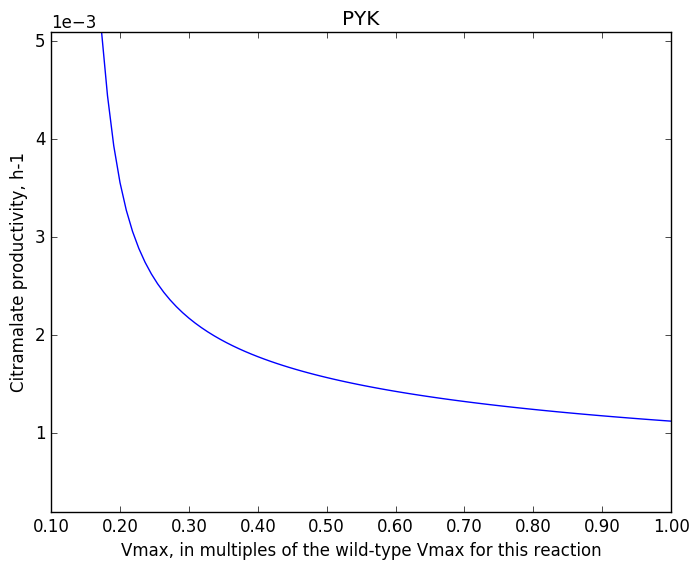
\includegraphics[scale=0.5]{onereacsample}
  \caption{Example of a one-reaction plot, the reaction PYK}
  \label{fig:onereacsample}
\end{figure}

Some reactions showed greater changes in citramalate productivity as $V_{max}$ changed. I quantified these effects by taking the difference between the maximum and minimum productivity values obtained for each reaction as $V_{max}$ was varied over the 0.5 -- 2.0 $V_{max}$ range.  Using these difference values, I ordered the reactions into a `one-reaction list' (appendix~\ref{ap:onereactionlist})

The one-reaction list identified CITRA\_SYN, GLT, LPD, GROWTH, ATP\_MAIN\-TEN\-ANCE, GDH, ATP\_SYN, ACEA, PYK, and ZWF as reactions that had the greatest effects on citramalate productivity.
The exchange reactions (XCH\_ACE, XCH\_GLC, and XCH\_P) had no bearing on productivity; all the data points in their plots could be attributed to noise. Surprisingly, the reactions that directly concern acetyl CoA -- ACS, ACK, and PTA -- did not seem to have conspicuous bearings on productivity.

Additionally, some reactions had inflection points (table~\ref{tab:inflection}). These inflection points could complicate finding $V_{max}$ combinations to optimise citramalate productivity.

\begin{table}[!htbp]
  \caption{Reactions that exhibited inflection points in citramalate productivity as a function of $V_{max}$. Values listed are the values at inflection points}
  \label{tab:inflection}
  \centering
  \begin{tabular}{lrrl}
    \toprule
    Reaction & $V_{max}$ (mM s\textsuperscript{-1}) & Productivity (h\textsuperscript{-1}) & Type\\
    \midrule
    ATP\_syn & 16.804 & 0.00216 & local minimum\\
    & 23.724 & 0.00231 & local maximum\\
    CITRA\_SYN & 0.545 & 0.01660 & local maximum\\
    CYTBO & 5.124 & 0.00113 & local maximum\\
    EDA & 0.014 & 0.00112 & local maximum\\
    GDH & 4.569 & 0.00149 & local maximum\\
    MQO & 1.597 & 0.00098 & local minimum\\
    PFK & 0.145 & 0.00113 & local maximum\\
    \bottomrule
  \end{tabular}
\end{table}

%In addition, I also extracted a list of reactions arranged by descending order of flux control coefficient (FCC) from the Millard \emph{et al.} paper, and used it alongside the one-reaction list in later parts of the project.

\section{Varying $V_{max}$ values two reactions at a time}
\label{sec:couples}

Varying $V_{max}$ values of two reactions at a time aimed to identify pairs of reactions that had significant effects on citramalate productivity. This is a stepping stone to identifying the optimal conditions. Ideally, all possible pairs should be investigated. However, I used only the eight reactions at the top of the one-reaction list: CITRA\_SYN, GLT, LPD, ATP\_MAINTENANCE, GDH, ATP\_syn, ACEA, and ZWF. This is to save computation time and to focus on the most useful output. I varied the reactions' $V_{max}$ values within 0.1--10.0 $V_{max}$, and plotted the resulting citramalate productivities on heatmaps (figure~\ref{fig:heatmapsample}). %The $V_{max}$ values took 10 values in their ranges, so each heatmap had 100 data points. Because the wild-type productivity is 0.001122 h\textsuperscript{-1}, I multiplied the citramalate productivity values by 10,000 so that numbers that can be easily conceptualised are displayed on the heatmaps. In figure~\ref{fig:heatmapsample}, when the $V_{max}$ of GLT is 256.76 mM s\textsuperscript{-1} and the $V_{max}$ of ACEA is 1.83 mM s\textsuperscript{-1}, productivity is 0.00848 h\textsuperscript{-1}.

\begin{figure}[!htbp]
  \centering
  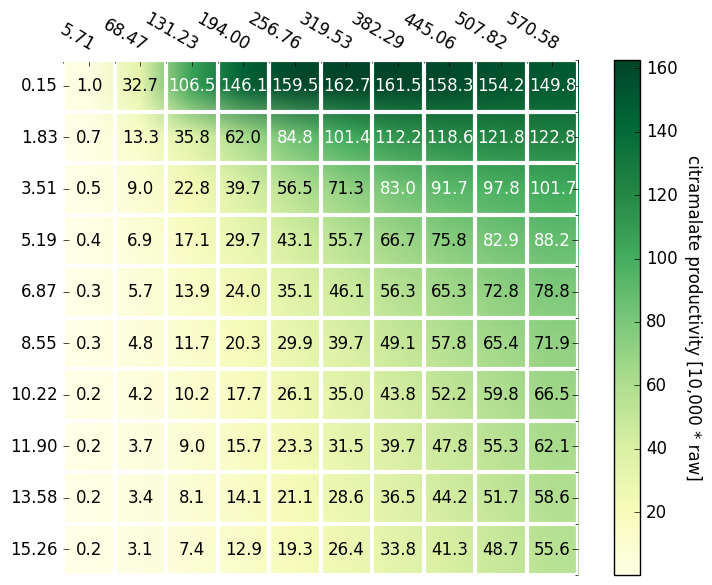
\includegraphics[scale=0.5]{heatmapsample}
  \caption{Example of a heatmap: GLT vs ACEA. The horizontal axis indicates the respective $V_{max}$ value of the first reaction (GLT) in mM s\textsuperscript{-1} and the vertical axis represents the second reaction (ACEA). Citramalate productivity ($\times${}10,000 h\textsuperscript{-1}) values are displayed.}
  \label{fig:heatmapsample}
\end{figure}

% I also used the reactions with the 10 greatest FCCs to generate heatmaps.
Most heatmaps suggested simple additive effects. The heatmaps had the same local minima and maxima as with investigating single reactions, thus suggesting orthogonality. Plots that involved ATP\_MAIN\-TEN\-ANCE exhibited strange behaviour, evident in higher-resolution heatmaps (figure~\ref{fig:atpmaintenanceheatmap}). Possibly, the kinetic model was not configured well for small values of $V_{max}$, (figure~\ref{fig:atpmaintenanceonereac}).

\begin{figure}[hp]
  \centering
  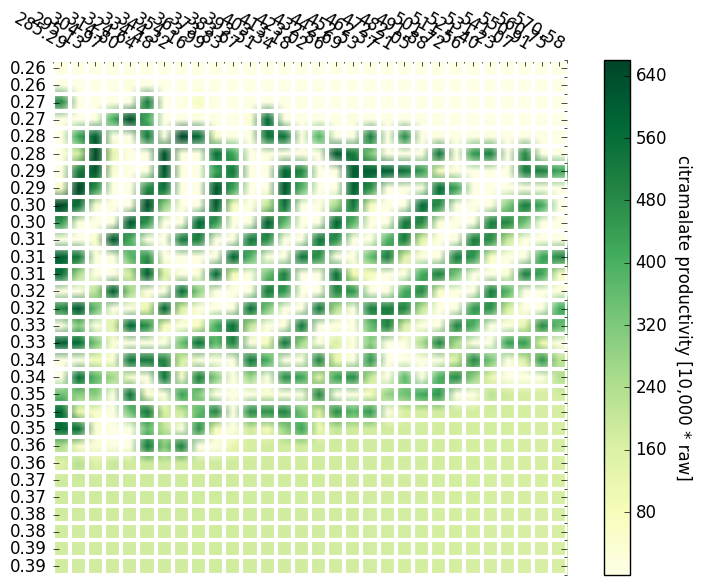
\includegraphics[scale=0.5]{atpmaintenanceheatmap}
  \caption{High-resolution heatmap of GLT vs ATP\_MAINTENANCE}
  \label{fig:atpmaintenanceheatmap}

  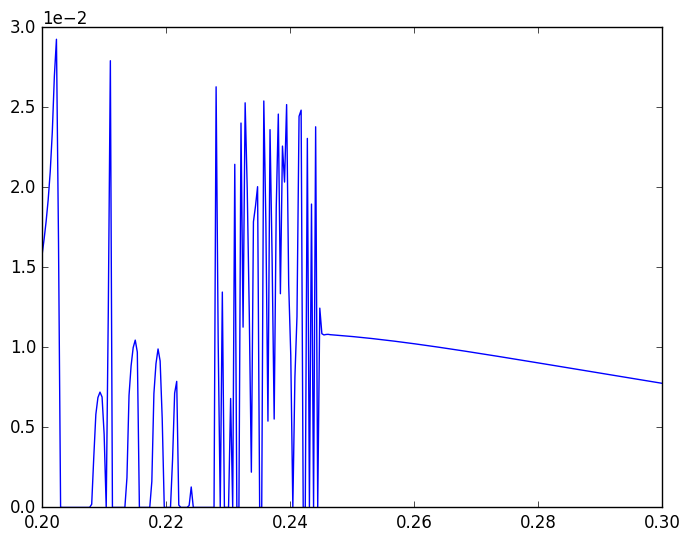
\includegraphics[scale=0.5]{atpmaintenanceonereac}
  \caption{One-reaction plot for ATP\_MAINTENANCE, 300 data points}
  \label{fig:atpmaintenanceonereac}
\end{figure}

\subsection{Steady-state verification}
\label{ssec:steadystate}

The results are only valid if the system has reached steady state, as the focus is on continuous cultures and the project aims to enrich a stoichiometric model. Steady state is achieved if at the end of simulation time:

\begin{equation}
  \max_{X_{i}} \left | \frac{\mathrm{d}[X_{i}]}{\mathrm{d}t} \right | < \epsilon
\end{equation}
\label{eqn:steadystate}

where $X_{i}$ represents a chemical species, and $\epsilon$ is a small threshold value. Heatmaps aided this validation (figure~\ref{fig:steadystate}).

\begin{figure}[hbp]
  \centering
  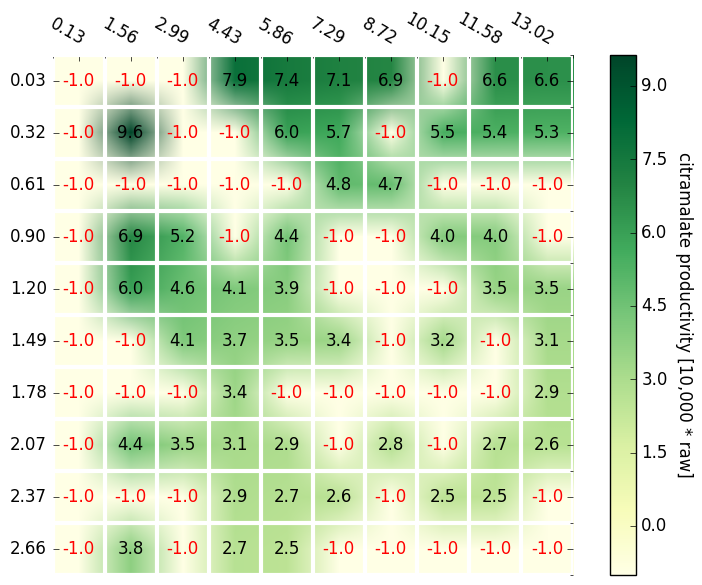
\includegraphics[scale=0.5]{steadystate}
  \caption{Heatmap for GLT vs ZWF, with threshold set to \num{1.0e-6} mM s\textsuperscript{-1}. Data points are replaced by -1 if the system does not reach steady state.}
  \label{fig:steadystate}
\end{figure}

%In most cases, ATP, ADP, P, or Hout was responsible for breaking the \num{1.0e-8} threshold. However, their rates stayed at around \num{1.0e-7}.

In almost all cases, the model was confirmed to have reached steady state using \num{1.0e-6} mM s\textsuperscript{-1} as the threshold. However, ATP\_MAIN\-TEN\-ANCE set at 0.1 $V_{max}$ produced maximum concentration change rates at the order of \num{e-1} mM s\textsuperscript{-1}, and ATP\_syn set at 0.1 $V_{max}$ produced rates at the order of \num{e-2} mM s\textsuperscript{-1}. With these two reactions, the species responsible for breaking the threshold were BPG and OAA.
Finally, GDH set at 0.1 $V_{max}$ produced rates on the order of \num{e-3} mM s\textsuperscript{-1}, with GLCx and GLCp responsible for breaking the threshold. This was the only situation where GLCx and GLCp concentrations did not reach steady state.

\section{Using differential evolution to vary $V_{max}$ values of multiple reactions}
\label{sec:de}

Differential evolution is a genetic algorithm developed by \citet{storn_differential_1997}. I used the \texttt{rand/1/bin} strategy, adapting code by \citet{mier_tutorial_2017, mier_small_2017}.

Differential evolution includes the following parameters:
\begin{itemize}
\item $F$, the mutation constant or differential weight;
\item $CR$, the recombination constant or crossover probability;
\item $NP$, the population size; and
  \item $D$, the number of dimensions, equal to the number of reactions investigated simultaneously.
\end{itemize}
The number of iterations must also be specified.

In this section, I used citramalate productivity calculated after \texttt{roadrunner} simulations as the objective function to be maximised. $V_{max}$ values of multiple reactions in a specified list were varied simultaneously.

Using parameter values suggested by \citet{storn_differential_1997} ($F$ = 0.8, $CR$ = 0.3, $NP$ = 20, 20 iterations), differential evolution agreed with heatmaps in identifying the $V_{max}$ values that optimised productivity.
For example, the GLT vs ACEA heatmap (figure \ref{fig:heatmapsample}) estimated that the maximal productivity from varying the $V_{max}$ values of these two in the 0.1 -- 10.0 $V_{max}$ range is \num{162.7e-4} h\textsuperscript{-1} and occurs when the GLT $V_{max}$ is 319.53 mM s\textsuperscript{-1} and the ACEA $V_{max}$ is 0.15 mM s\textsuperscript{-1}. Differential evolution indicated that the maximal productivity is \num{162.7e-4} h\textsuperscript{-1} and occurs when the GLT $V_{max}$ is 325.6 mM s\textsuperscript{-1} and the ACEA $V_{max}$ is 0.1526 mM s\textsuperscript{-1}.
% would be better if we had a more thorough investigation of ALL heatmaps, but this should be fine...?
Occasionally, differential evolution discovered maxima not evident in the heatmaps, but this could be explained by the relatively low resolution of the heatmaps. 

\subsection{Finding optimal differential evolution parameters}
\label{ssec:deoptimise}

I tested how well the suggested \citep{storn_usage_1996, pedersen_good_2010} differential evolution parameter values optimised citramalate productivity. I used reactions in the glycolytic pathway and the one-reaction list. Values were chosen based on algorithm run time and how fast convergence was realised. They are presented in table~\ref{tab:deoptimise}.

\begin{table}[h]
  \caption{Development of optimal parameters for using differential evolution with the kinetic model}
  \label{tab:deoptimise}
  \centering
  \begin{tabularx}{\linewidth}{LLLLLLL}
    \toprule
    $F$ & $CR$ & $NP$ & iterations & $D$ & Source\\
    \midrule
    0.8 & 0.7 & 20 & & 2-3 & Mier\\
    0.8 & 0.7 & 20 & 25-40 & 5 & Mier\\
    0.6 & 0.9 & \textless 40 & \textgreater 20 & 5 & Storn\\
    0.6301 & 0.7122 & 17 & 50 & 6-7 & Pedersen (D = 5)\\
    0.6301 & 0.7122 & 17 & 70 & 7 & Pedersen (D = 5)\\
    0.6607 & 0.9426 & 28 & 50 & 7-10 & Pedersen (D = 10, first set), best\\
    0.6702 & 0.2368 & 12 & 100 & 7 & Pedersen (D = 10, second set)\\
    \bottomrule
  \end{tabularx}
\end{table}

\subsection{Optimisation of citramalate production}
\label{ssec:optcitra}

Using the best differential evolution parameters ($F$ = 0.6607, $CR$ = 0.9426, $NP$ = 28, and 50 iterations) with the set of seven reactions -- CITRA\_SYN, GLT, LPD, GDH, ATP\_syn, ACEA, and ZWF -- varying $V_{max}$ values over 0.1--10.0 $V_{max}$ yielded optimal $V_{max}$ values for each reaction (table~\ref{tab:optcitra7}) and the citramalate productivity of \num{353.66e-4} h\textsuperscript{-1}.

I verified these findings by manually setting the $V_{max}$ values of these seven reactions. For each reaction, I chose the $V_{max}$ value within the 0.1 -- 10.0 $V_{max}$ range that corresponds to the greatest citramalate productivity as found in section~\ref{sec:onereac}; the $V_{max}$ value of each reaction was set independently of all other reactions. The simulation returned the productivity of \num{226.96e-4} h\textsuperscript{-1}, lower than the productivity found from differential evolution. This thus confirms that differential evolution is useful.

\begin{table}[hp]
  \caption{Optimal $V_{max}$ values, using seven reactions from the one-reaction list}
  \label{tab:optcitra7}
  \centering
  \begin{tabular}{lSl}
    \toprule
    Reaction & \multicolumn{1}{c}{Optimal $V_{max}$ (mM s\textsuperscript{-1})} & Remark\\
    \midrule
    CITRA\_SYN & 0.4382 & \\
    GLT & 5.706 & 0.1 $V_{max}$ \\
    LPD & 0.006844 & 0.1 $V_{max}$ \\
    GDH & 3.591 & \\
    ATP\_syn & 10.87 & 0.1 $V_{max}$ \\
    ACEA & 0.1526 & 0.1 $V_{max}$ \\
    ZWF & 0.02658 & 0.1 $V_{max}$\\
    \bottomrule
  \end{tabular}
\end{table}

Furthermore, I tried the same differential evolution parameters on 10 enzymes (table~\ref{tab:optcitra10}) and achieved the productivity of \num{405.5e-4} h\textsuperscript{-1}. However, 10 reactions showed slower convergence, as expected by the `curse of dimensionality'. This `curse' is a limitation of differential evolution in which the difficulty of finding solutions increases exponentially as dimensions increase.

\begin{table}[hp]
  \caption{Optimal $V_{max}$ values, using ten reactions from the one-reaction list}
  \label{tab:optcitra10}
  \centering
  \begin{tabular}{lSl}
    \toprule
    Reaction & \multicolumn{1}{c}{$V_{max}$ in best solution (mM s\textsuperscript{-1})} & Range\\
    \midrule
    CITRA\_SYN & 1.689 & \\
    GLT & 17.35 & 0.1 $V_{max}$ \\
    LPD & 0.007174 & $\approx$ 0.006844 \\
    GDH & 0.8910 & 0.08666 $\sim$ 0.08910\\
    ATP\_syn & 10.87 & 10.87 $\sim$ 13.01 \\
    ACEA & 0.1826 & 0.1529 $\sim$ 0.01826 \\
    PYK & 0.007472 & $\approx$ 0.007472 \\
    ZWF & 0.02658 & always 0.02658 \\
    NDHII & 10.45 & \\
    MQO & 0.4623 & almost always 0.4623\\
    \bottomrule
  \end{tabular}
\end{table}

I repeated the investigation using the ten enzymes with the greatest flux control coefficients (table~\ref{tab:optfcc10}). In this case, the productivity was \num{224.2e-4} h\textsuperscript{-1}. I excluded ATP\_MAINTENANCE because it does not correspond to an enzyme that exists in \emph{E. coli} and because it was not reliable with small values of $V_{max}$, as discussed in section~\ref{sec:onereac}.

\begin{table}[hp]
  \caption{Optimal $V_{max}$ values, using ten reactions with the greatest FCCs}
  \label{tab:optfcc10}
  \centering
  \begin{tabular}{lSl}
    \toprule
    Reaction & \multicolumn{1}{c}{Optimal $V_{max}$ (mM s\textsuperscript{-1})}\\
    \midrule
    CYTBO & 3.416 \\
    MQO & 1.849 \\
    MDH & 61.15 \\
    ZWF & 0.1072 \\
    GLT & 378.7 \\
    GDH & 4.485 \\
    ATP\_syn & 43.49 \\
    ACK & 20.15 \\
    ACEA & 0.6189 \\
    EDD & 0.6605\\
    \bottomrule
  \end{tabular}
\end{table}

Using all 41 biologically relevant reactions that had $V_{max}$ as a parameter did not exhibit enough convergence due to the high number of dimensions. However, this produced productivities on the order of \num{200e-4} h\textsuperscript{-1} every time the algorithm was repeated, which was still a significant improvement from wild-type productivity.
\subsection{Glycolytic enzymes}
\label{ssec:glycolytic}

%Originally I used differential evolution with the glycolytic enzymes PGI, PFK, FBA, GDH, PGK, GPM, ENO, PYK, and PDH to investigate whether the $V_{max}$ values of all enzymes in a pathway must be increased for an appreciable increase in the overall flux through the pathway, leading to higher productivity. From their experiments on the tryptophan synthesis pathway in yeast, \citet{niederberger_strategy_1992} concludes that the fluxes through each enzyme in a linear pathway must all be increased to increase the flux through the pathway. However, \cite{yamamoto_overexpression_2012} show that appreciable increases result after increasing the flux through only one or two enzymes. My results, included in \texttt{kinetic/result/de/gly.txt} support the latter.

I investigated how much adding reactions as additional dimensions in differential evolution affected the use of the algorithm to optimise citramalate productivity. I used differential evolution in a similar fashion as earlier, but on the glycolytic enzymes that are arranged in a linear fashion --  PGI, PFK, FBA, GDH, PGK, GPM, ENO, PYK, and PDH.

Initially, I varied the $V_{max}$ values of a smaller set of reactions in the process of differential evolution. Then, I varied the $V_{max}$ values of a larger set of reactions, which included enzymes that I have identified as having less of an effect on citramalate productivity (i.e. lower on the one-reaction list, appendix~\ref{ap:onereactionlist}).

Specfically, at first I ran differential evolution using the five enzymes PGI, GDH, ENO, PYK, and PDH. This resulted in the citramalate productivity of \num{269.72e-4} h\textsuperscript{-1} (20 iterations). Then, I added PFK to create the set of six enzymes PGI, GDH, ENO, PYK, and PDH, and optimised citramalate productivity in the same way, and so on. Adding PFK (23rd on the one-reaction list), FBA (29th), and GPM (25th) returned \num{290.04e-4} h\textsuperscript{-1} ($D$ = 8, $F$ = 0.6607, $CR$ = 0.9426, $NP$ = 28, 50 iterations). Finally, when PGK (44th) was added, the simulations never managed to achieve a productivity that exceeded the previous.

Thus, adding enzymes deemed to have less of an effect on citramalate producitivty had little effect on the optimum $V_{max}$ values found earlier, and did not cause large improvements in productivity.

\section{Glucose uptake}
\label{sec:glucoseuptake}

%% [Just revised this section, but it's still pretty shit. This section can just go if it isn't really used with the Lund medium later. Or figure out a way to link this with the Lund medium thing]

I investigated the kinetic model to determine whether there was decoupling between the glucose exchange and glucose uptake reactions.
Specifically, I examined the relationship between glucose feed and the fluxes through the other reactions in the kinetic model. I varied the flux through GLC\_feed and observed the following (figures~\ref{fig:growthglc_XCHGLCvGLCfeed} and \ref{fig:growthglc_species}):

\begin{itemize}
\item Fluxes through XCH\_GLC and all PTS\_X reactions were equal to each other, until GLC\_feed exceeded 0.82 mM s\textsuperscript{-1}, at which the flux through XCH\_GLC slightly exceeded that of the PTS\_X reactions.
\item Flux through XCH\_GLC increased linearly with GLC\_feed until the value of 0.82 mM s\textsuperscript{-1}, after which it plateaued.
\item GLCx and GLCp concentrations remained very low as GLC\_feed flux increased up to 0.82 mM s\textsuperscript{-1}. After that, their concentrations increased linearly as GLC\_feed flux increased
\item The concentration of G6P increased linearly as GLC\_feed flux increased up to 0.82 mM s\textsuperscript{-1}, at which the concentration immediately plateaued at 3.19 mM.
  \item Concentrations of all metabolites except for CITRA were at steady-state when GLC\_feed was below 0.82 mM s\textsuperscript{-1}. At any GLC\_feed value over 0.82 mM s\textsuperscript{-1}, GLCx and GLCp concentrations were increasing with respect to time (i.e. \( \dv{GLCp}{t} > 0, \dv{GLCx}{t} > 0\)).
\end{itemize}

\begin{figure}[hp]
  \centering
  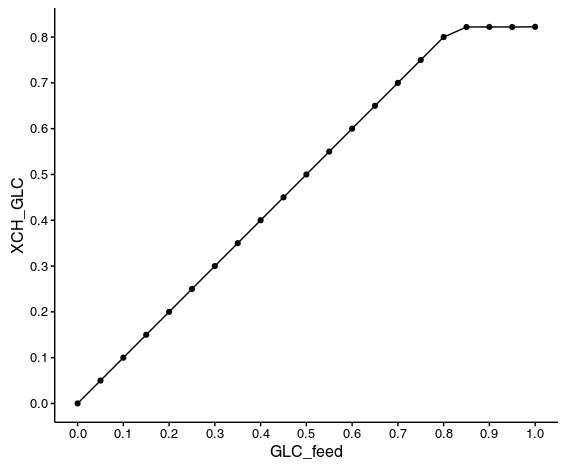
\includegraphics[scale=0.5]{growthglc_XCHGLCvGLCfeed}
  \caption{Effect of GLC\_feed on XCH\_GLC; XCH\_GLC values are equal to that of PTS\_0 to PTS\_4}
  \label{fig:growthglc_XCHGLCvGLCfeed}

  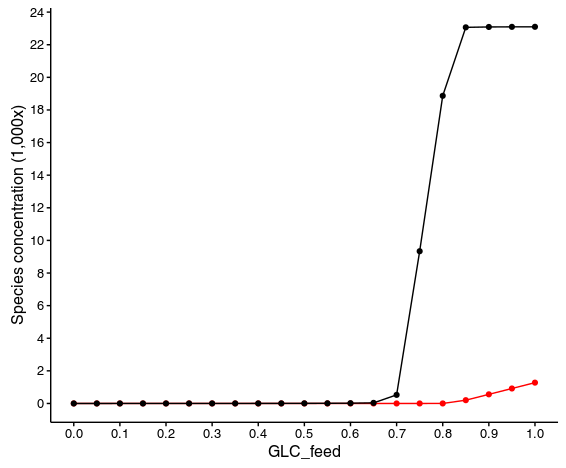
\includegraphics[scale=0.5]{growthglc_species}
  \caption{Effect of GLC\_feed on concentrations of various species; red is GLCx = GLCp, black is G6P}
  \label{fig:growthglc_species}
\end{figure}

%% [Perhaps put this in discussion???]
Results suggested that the model did not predict decoupling between glucose exchange and glucose uptake; however, glucose exchange reached saturation.
Information about such decoupling relates to the relationship between the intracellular and extracellular concentrations of glucose. This relationship would be useful in determining the effects of a nutrient medium containing glucose on citramalate productivity.

\chapter{Enriching the stoichiometric model}
\label{ch:stoich}

The stoichiometric model consists of reaction stoichiometries along with lower and upper bounds for flux for each reaction. These bounds can be specified to provide constraints for FBA.% Using linear programming, FBA aims to find an optimal solution for an objective function, subject to constraints on flux values. The objective function can be minimised or maximised, and this can be specified when using \texttt{cobra} to compute the solutions. 
\section{Creating boundaries for flux balance analysis}
\label{sec:bounds}

The lowest and highest possible values of fluxes through each reaction in the kinetic model provides reasonable bounds for the stoichiometric model.
To find the lowest and highest possible flux values through the 69 reactions of the kinetic model, I varied the $V_{max}$ values of the 49 reactions with $V_{max}$ as a parameter, CITRA\_SYN included.

Initially, to save computation time, I varied $V_{max}$ values of one reaction at a time over the range of 0.1-10.0 $V_{max}$, and recorded the minimum and maximum flux values achieved for each reaction after simulations. These produced a set of flux bounds I term `one-dimension bounds' (data not shown).
% This is not supported by `hard' data yet, but it's better than nothing. Will improve this later.
In subsequent investigations, I found out the that difference between the computed upper and lower bounds is decreased with smaller ranges for $V_{max}$ values. Furthermore, the bounds are most sensitive over the range of 0.1-3.0 $V_{max}$

Then, I used differential evolution to find the lowest and highest possible fluxes through each kinetic model reaction. The simulated flux through each reaction was the objective function. To calculate the lower bound for each reaction, this objective function was minimised, and to calculate the upper bound, it was maximised.

First, I included the eight reactions with the greatest flux control coefficients: CYTBO, MQO, MDH, ZWF, GLT, GDH, ATP\_syn, and ACK, with parameters $F$ = 0.6607, $CR$ = 0.9426, $NP$ = 28, and 5 iterations \citep{pedersen_good_2010}. I used the $V_{max}$ range of of 0.3--10.0 $V_{max}$ because $V_{max}$ values less than 0.3 $V_{max}$ tended to produce run time errors in \texttt{roadrunner} in which convergence test failures occurred too many times. Using this restricted range was justified by the aberrant behaviour of ATP\_MAINTENANCE (section~\ref{sec:couples}), which suggested that the model was not reliable with such small $V_{max}$ values. From this work, I produced `eight-dimension bounds' (data not shown). Increasing the number of iterations to 20 only marginally broadened the bounds.

Second, I included all 41 enzyme-catalysed reactions in the kinetic model with $V_{max}$ as a parameter. Here, I used the differential evolution parameters of $F$ = 0.6876, $CR$ = 0.9784, $NP$ = 48 \citep{pedersen_good_2010}, and five iterations. To avoid convergence test failures, I set the $V_{max}$ range to 0.5--10.0 $V_{max}$. From this, I produced `41-dimension bounds' (appendix~\ref{ap:41dbounds}).

The 41-dimension bounds were mostly wider than both one- and eight-dimension bounds. 41-dimension lower bounds were the most negative among the three sets for 43 of 57 reactions, and 41-dimension upper bounds were the most positive for 42 out of 57 reactions.

\section{Mapping reactions in the kinetic model to the stoichiometric model}
\label{sec:mapping}

Previously (before June 2018), an Anargyros who worked in this group produced a mapping table which mapped reactions in the kinetic model to reactions in the stoichiometric model. %Flux bounds were also included, but the method by which the bounds were generated had not been documented and no specific constraints had been used.
I improved on this mapping table by correcting errors, re-defining relationships between kinetic and stoichiometric model reactions, re-calculating flux bounds, and reconciling differing sub-network structures between the two models.

The current (20 September 2018) mapping table (appendix \ref{ap:mapping})
concerns the 68 reactions present in the wild-type kinetic model, including the growth reaction. The full mapping table included:
\begin{itemize}
\item Kinetic and stoichiometric model reaction IDs and stoichiometries, plus stoichiometric model reaction names
  \item EC numbers for kinetic model reactions quoted by \citet{millard_metabolic_2017} and EC number for stoichiometric model reactions extracted from the respective SBML file
\item Categorisation of reactions into sub-systems as specified by \citet{millard_metabolic_2017}
  \item Relationships and differences between stoichiometric model reactions and the corresponding kinetic model reactions
\end{itemize}

%% Commented this out because I'm focussing on the end result more than development that no-one will care about in this extended report. I'm going to focus more on WHY things are the way they are

% I updated the mapping spreadsheet by correcting mistakes and mapping more enzymes. Table~\ref{tab:mapping} presents the mapping changes I made to correct the mistakes.

% \begin{table}[htb]
%   \label{tab:mapping}
%   \caption{Changes to mapping pairs in the mapping table}
%   \centering
% \begin{tabularx}{\linewidth}{|L|L|L|}
%   \hline
%   \bfseries Before & \bfseries After & \bfseries Notes\\
%   \hline
%   Kinetic MDH $\rightarrow$ Stoich MDH2 & Kinetic MDH $\rightarrow$ Stoich MDH, and the reactions are reversed with respect to each other. & Corrected confusion between types of malate dehydrogenases. Re-mapping judged from EC numbers and substrates in the reactions\\
%   \hline
%   Kinetic XCH\_GLC $\rightarrow$ Stoich GLCtexi & Kinetic XCH\_GLC $\rightarrow$ Stoich GLCtex & Chose a reversible reaction to replace an irreversible one\\
%   \hline
%   Kinetic XCH\_ACE2 $\rightarrow$ Stoich ACACtex & Kinetic XCH\_ACE2 $\rightarrow$ Stoich ACtex & Corrected a mistake -- it's acetate exchange, not acetoacetate exchange\\
%   \hline
% \end{tabularx}
% \end{table}

Three reactions are absent in the stoichiometric model (GL6P\_HYDROLYSIS, ACEK\_1, and ACEK\_2), so the fluxes of these reactions were ignored in the mapping. Additionally, stoichiometric CYTBO3\_4pp has a different stoichiometry from kinetic CYTBO. Furthermore, the growth reactions from the two models use different coefficients.

Fifteen reactions are identical between the kinetic and stoichiometric model. Reactions that are not identical fall into the following categories:

\begin{enumerate}
\item \emph{Plus small chemical species:} reactions that are otherwise identical, but differ by the addition of the species \ce{H^+} or \ce{H2O}
\item \emph{Acid hydrolysis:} reactions that are otherwise identical, but \ce{CO2} is listed in the stoichiometric model in place of \ce{HCO3^-}
\item \emph{Different reversibility:} reactions that are otherwise identical, but are reversible in the stoichiometric model with its counterpart in the kinetic model being irreversible, or vice versa
\item \emph{Reversed:} reactions that are reversed with respect to one another
  \item \emph{Sub-network different structure:} reactions that belong to sub-networks that are structured differently and therefore do not allow one-to-one mapping; these include the glucose uptake and the pentose phosphate pathway sub-systems
  \end{enumerate}

I devised rules to map flux values from the kinetic model onto the stoichiometric model. For categories 1--3, stoichiometric model reactions have the same lower and upper flux bounds as their kinetic model counterparts. For category 4, the values were negated -- i.e. $ \mathrm{Kinetic } (lb, ub) \rightarrow \mathrm{Stoichiometric } (-ub, -lb)$. %note: might need overfull hbox fixes/bodges depending on how this looks like in the final version

Reactions in category 5 demanded special treatment. Their architectures in the two models are summarised in figures~\ref{fig:glucoseuptake} and~\ref{fig:ppp}.

\begin{figure}[!p]
  \centering
  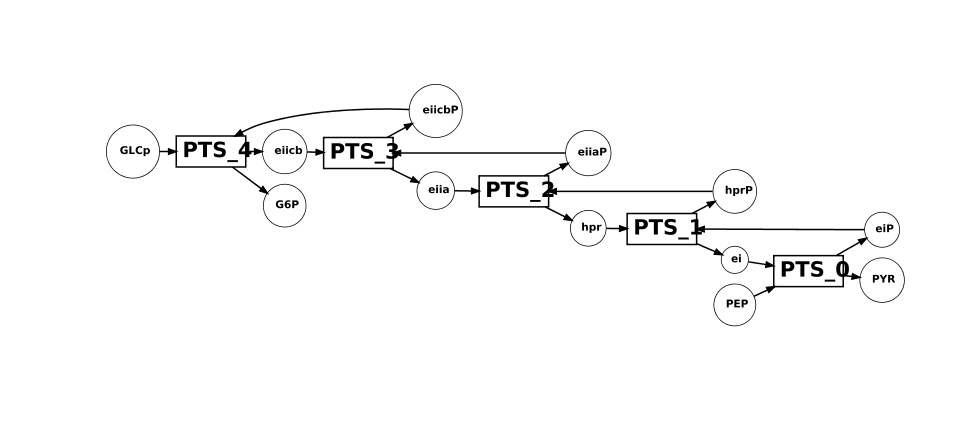
\includegraphics[scale=0.4]{glucoseuptake}
  \caption{Sub-network for glucose uptake}
  \label{fig:glucoseuptake}
\end{figure}

\begin{figure}[!p]
  \centering
  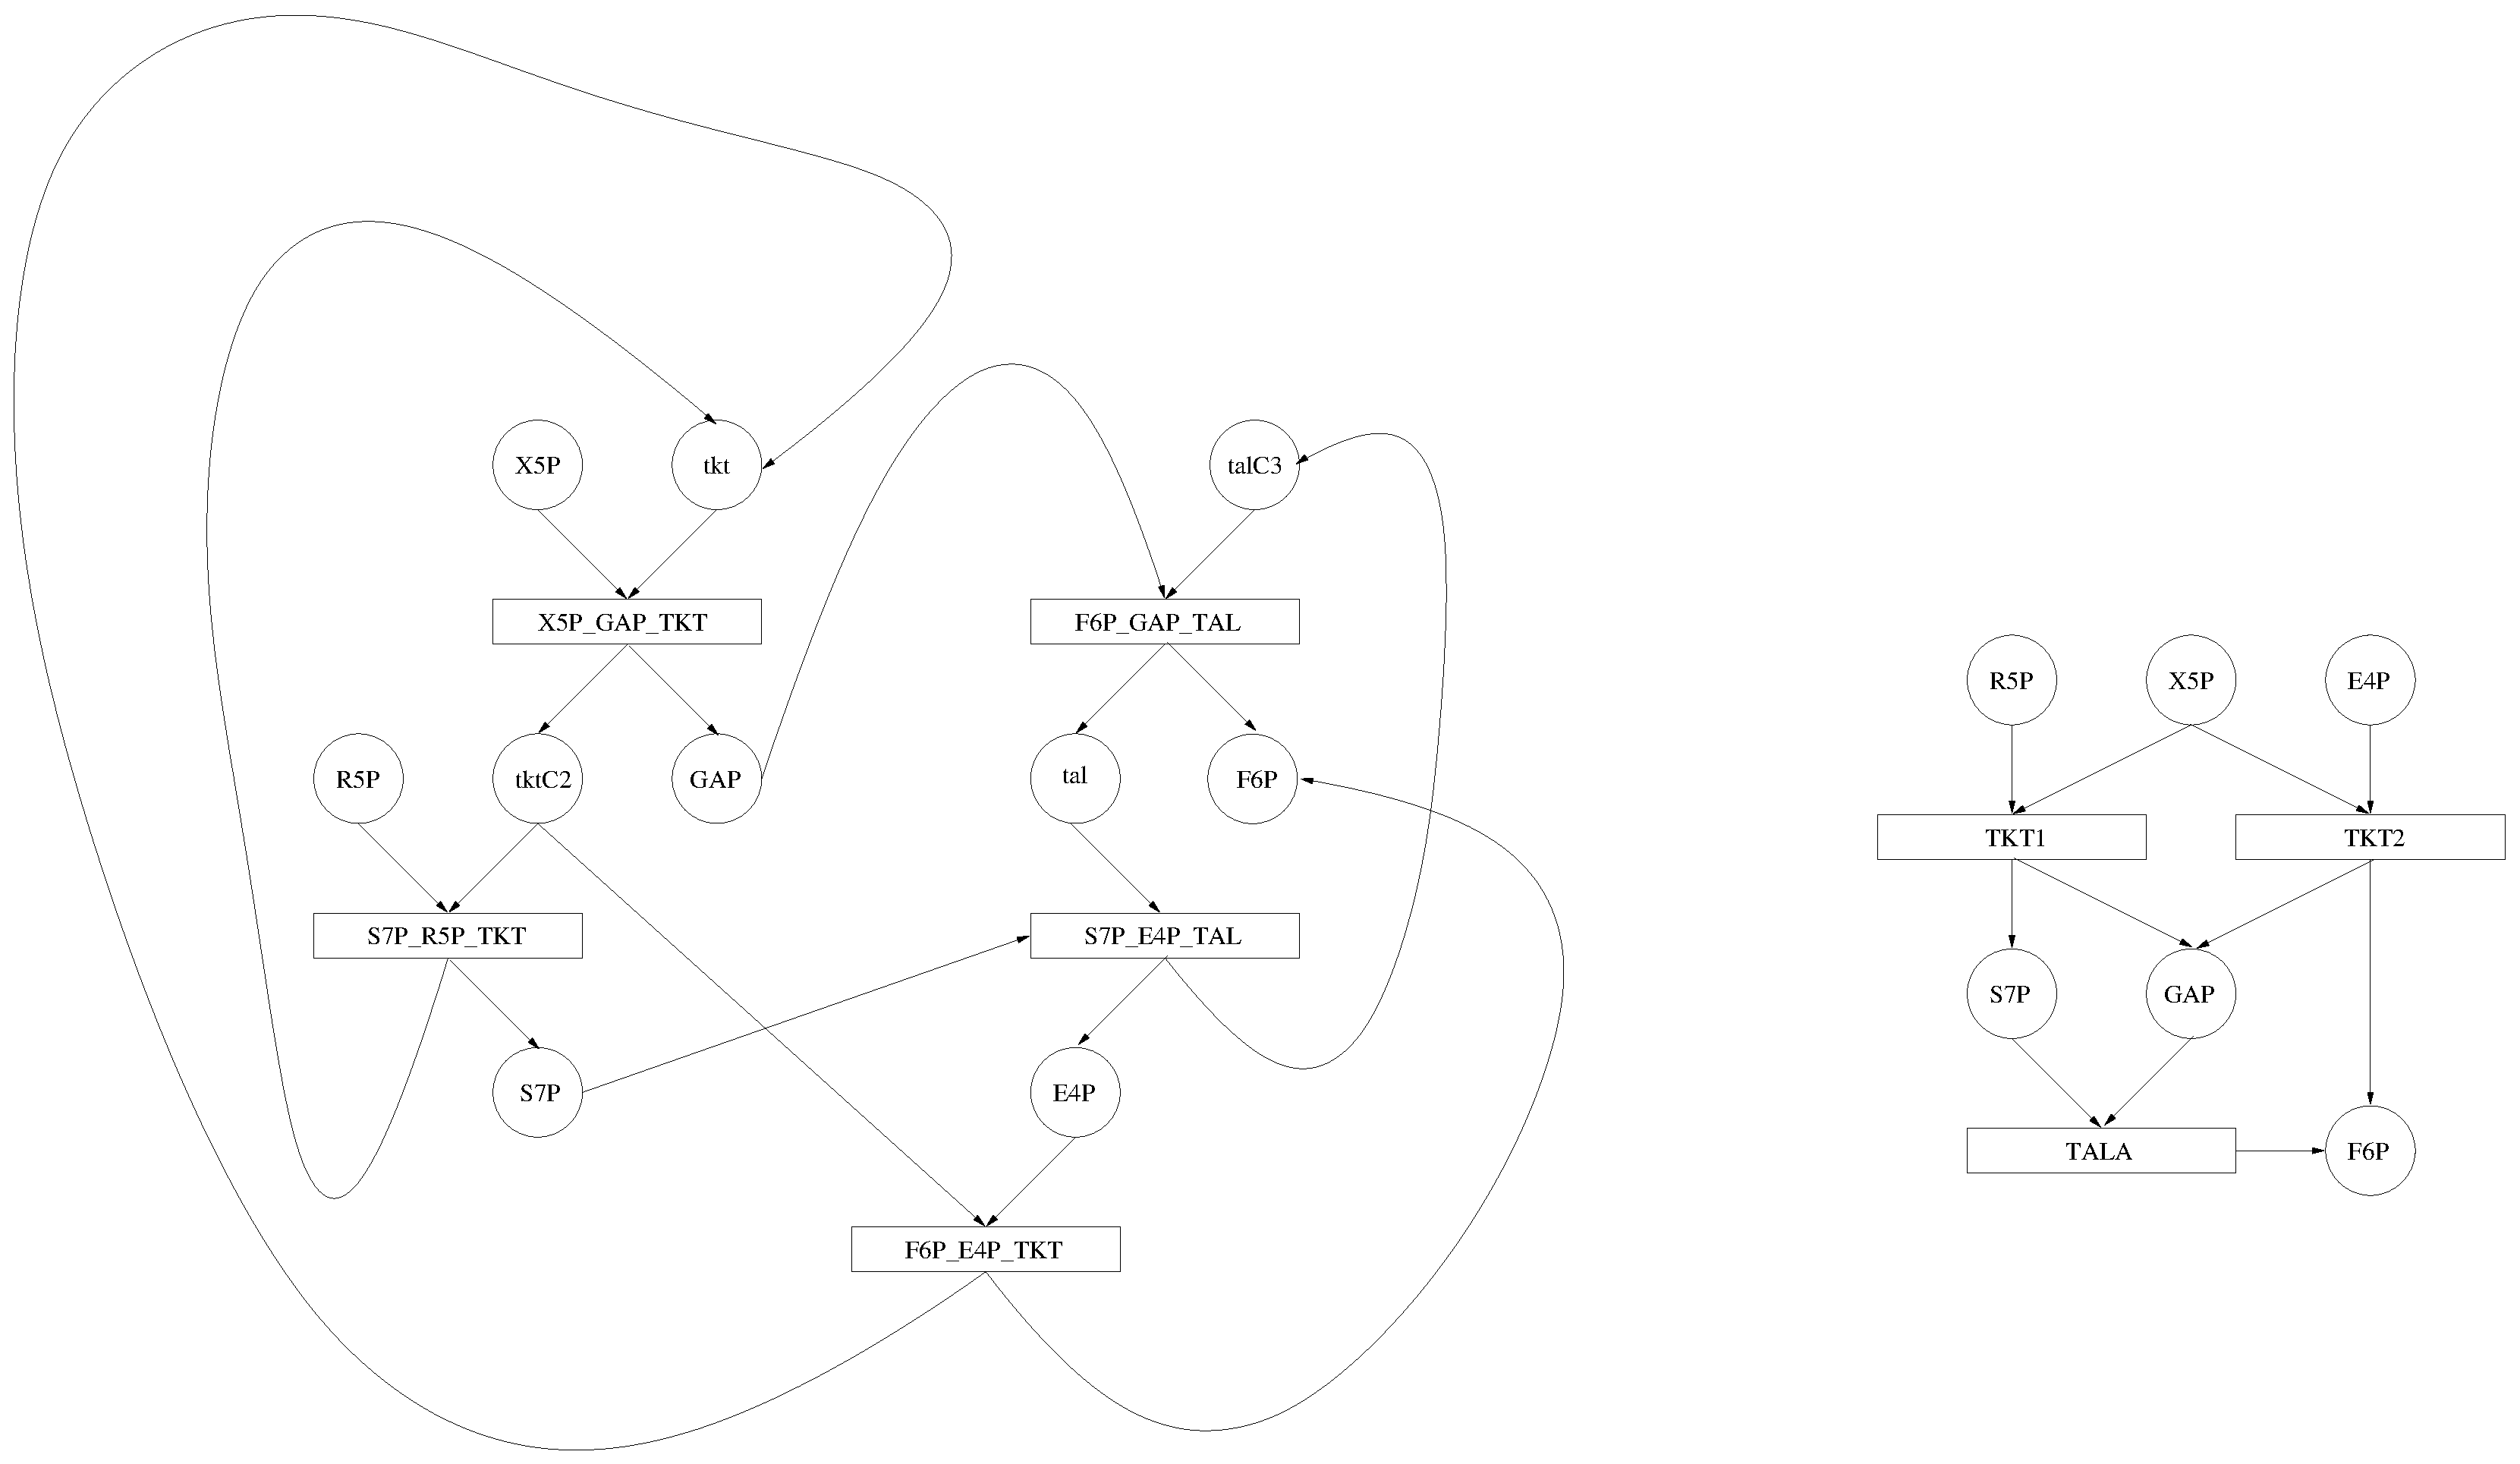
\includegraphics[scale=0.25]{ppp}
  \caption{Sub-network for part of the pentose phosphate pathway; left - kinetic model, right - stoichiometric model}
  \label{fig:ppp}
\end{figure}

I mapped glucose uptake reactions according to table~\ref{tab:glucoseuptake}. Mapping GLC\_feed to EX\_glc\_(e) is based on how both correspond to glucose feed into the environment, and mapping XCH\_GLC to GLCtex is based on the species involved on both sides of the reaction. However, mapping PTS\_0 to PTS\_4 to GLCptspp is based on investigating their behaviour in response to varying flux through GLC\_feed.

\begin{table}[!htbp]
  \caption{Mapping glucose uptake reactions}
  \label{tab:glucoseuptake}
  \centering
  \begin{tabularx}{\linewidth}{LLL}
    \toprule
    Kinetic model & Stoichiometric model & What it is\\
    \midrule
    GLC\_feed & EX\_glc\_(e) & Glucose feed (chemostat) into the environment\\
    XCH\_GLC & GLCtex & Glucose transport from environment to periplasm\\
    PTS\_0, PTS\_1, PTS\_2, PTS\_3, PTS\_4 & GLCptspp & Glucose uptake from periplam to cytoplasm\\
    \bottomrule
  \end{tabularx}
\end{table}

For the pentose phosphate pathway reactions, I focussed on each metabolite (X5P, GAP, R5P, S7P, F6P, and E4P) separately to determine the influx reactions (that produce the metabolite) and the outflux reactions (that consume the metabolite). I based the mapping on the principle that the sum of influxes in the kinetic model must be equivalent to the sum of influxes in the stoichiometric model, and that the same holds for outflux (figure~\ref{fig:pppmapping}).

\tikzstyle{met} = [draw, circle]
\tikzstyle{reac} = [rectangle]
\tikzstyle{line} = [draw, -latex']

\begin{figure}[h]
  \centering
  \begin{tikzpicture}[node distance = 1.5cm, every node/.style={scale=0.8}]
    % stoichiometric model metabolites
    \node [reac] (stolabel) {Stoichiometric model};
    \node [met, below of=stolabel] (x5psto) {X5P};
    \node [met, below of=x5psto] (gapsto) {GAP};
    \node [met, below of=gapsto] (r5psto) {R5P};
    \node [met, below of=r5psto] (s7psto) {S7P};
    \node [met, below of=s7psto] (f6psto) {F6P};
    \node [met, below of=f6psto] (e4psto) {E4P};
    %stoichiometric model reactions and arrows
    \node [reac, right of=x5psto, xshift=1.25cm] (x5psto-x5pgaptkt) {X5P\_GAP\_TKT};
    \path [line] (x5psto) -- (x5psto-x5pgaptkt);

    \node [reac, left of=gapsto, xshift=-1.25cm] (gapsto-x5pgaptkt) {X5P\_GAP\_TKT};
    \path [line] (gapsto-x5pgaptkt) -- (gapsto);    
    \node [reac, right of=gapsto, xshift=1.25cm] (gapsto-f6pgaptal) {F6P\_GAP\_TAL};
    \path [line] (gapsto) -- (gapsto-f6pgaptal);

    \node [reac, right of=r5psto, xshift=1.25cm] (r5psto-s7pr5ptkt) {S7P\_R5P\_TKT};
    \path [line] (r5psto) -- (r5psto-s7pr5ptkt);

    \node [reac, left of=s7psto, xshift=-1.25cm] (s7psto-s7pr5ptkt) {S7P\_R5P\_TKT};
    \path [line] (s7psto-s7pr5ptkt) -- (s7psto);    
    \node [reac, right of=s7psto, xshift=1.25cm] (s7psto-s7pe4ptal) {S7P\_E4P\_TAL};
    \path [line] (s7psto) -- (s7psto-s7pe4ptal);

    \node [reac, left of=f6psto, xshift=-1.25cm, yshift=0.25cm] (f6psto-f6pgaptal) {F6P\_GAP\_TAL};
    \node [reac, left of=f6psto, xshift=-1.25cm, yshift=-0.25cm] (f6psto-f6pe4ptkt) {F6P\_E4P\_TKT};
    \path [line] (f6psto-f6pgaptal) -- (f6psto);
    \path [line] (f6psto-f6pe4ptkt) -- (f6psto);    

    \node [reac, left of=e4psto, xshift=-1.25cm] (e4psto-s7pe4ptal) {S7P\_E4P\_TAL};
    \path [line] (e4psto-s7pe4ptal) -- (e4psto);    
    \node [reac, right of=e4psto, xshift=1.25cm] (e4psto-f6pe4ptkt) {F6P\_E4P\_TKT};
    \path [line] (e4psto) -- (e4psto-f6pe4ptkt);

    %kinetic model metabolites
    \node [reac, right of=stolabel, xshift=6cm] (kinlabel) {Kinetic model};
    \node [met, below of=kinlabel] (x5pkin) {X5P};
    \node [met, below of=x5pkin] (gapkin) {GAP};
    \node [met, below of=gapkin] (r5pkin) {R5P};
    \node [met, below of=r5pkin] (s7pkin) {S7P};
    \node [met, below of=s7pkin] (f6pkin) {F6P};
    \node [met, below of=f6pkin] (e4pkin) {E4P};
    %kinetic model reactions and arrows
    \node [reac, right of=x5pkin, xshift=0.5cm, yshift=0.25cm] (x5pkin-tkt1) {TKT1};
    \node [reac, right of=x5pkin, xshift=0.5cm, yshift=-0.25cm] (x5pkin-tkt2) {TKT2};
    \path [line] (x5pkin) -- (x5pkin-tkt1);
    \path [line] (x5pkin) -- (x5pkin-tkt2);

    \node [reac, left of=gapkin, xshift=-0.5cm, yshift=0.25cm] (gapkin-tkt1) {TKT1};
    \node [reac, left of=gapkin, xshift=-0.5cm, yshift=-0.25cm] (gapkin-tkt2) {TKT2};
    \node [reac, right of=gapkin, xshift=0.5cm] (gapkin-tala) {TALA};
    \path [line] (gapkin-tkt1) -- (gapkin);
    \path [line] (gapkin-tkt2) -- (gapkin);
    \path [line] (gapkin) -- (gapkin-tala);

    \node [reac, right of=r5pkin, xshift=0.5cm] (r5pkin-tkt1) {TKT1};
    \path [line] (r5pkin) -- (r5pkin-tkt1);

    \node [reac, left of=s7pkin, xshift=-0.5cm] (s7pkin-tkt1) {TKT1};
    \path [line] (s7pkin-tkt1) -- (s7pkin);    
    \node [reac, right of=s7pkin, xshift=0.5cm] (s7pkin-tala) {TALA};
    \path [line] (s7pkin) -- (s7pkin-tala);

    \node [reac, left of=f6pkin, xshift=-0.5cm, yshift=0.25cm] (f6pkin-tala) {TALA};
    \node [reac, left of=f6pkin, xshift=-0.5cm, yshift=-0.25cm] (f6pkin-tkt2) {TKT2};
    \path [line] (f6pkin-tala) -- (f6pkin);
    \path [line] (f6pkin-tkt2) -- (f6pkin);    

    \node [reac, left of=e4pkin, xshift=-0.5cm] (e4pkin-tala) {TALA};
    \path [line] (e4pkin-tala) -- (e4pkin);    
    \node [reac, right of=e4pkin, xshift=0.5cm] (e4pkin-tkt2) {TKT2};
    \path [line] (e4pkin) -- (e4pkin-tkt2);

  \end{tikzpicture}
  \caption{Rationale for mapping pentose phosphate pathways reactions between the kinetic and stoichiometric models}
  \label{fig:pppmapping}
\end{figure}


As a result, I produced the following rules:
\begin{itemize}
\item Kinetic X5P\_GAP\_TKT = Stoich.\ TKT1 + Stoich.\ TKT2 (from focussing on X5P and on GAP)
\item Kinetic F6P\_GAP\_TAL = Stoich.\ TALA (from focussing on GAP and on F6P)
\item Kinetic S7P\_R5P\_TKT = Stoich.\ TKT1 (from focussing on R5P and on S7P)
\item Kinetic S7P\_E4P\_TAL = Stoich.\ TALA (from focussing on S7P and on E4P)
  \item Kinetic F6P\_E4P\_TKT = Stoich.\ TKT2 (from focussing on F6P and on E4P)
  \end{itemize}

  This means that the lower bound of the sum of the fluxes of stoichiometric model TKT1 and stoichiometric model TKT2 is equal to the lower bound of kinetic model X5P\_GAP\_TKT, and the same applies to the upper bound. For the other reactions, the lower bound of the kinetic model reaction is equal to the upper bound of the corresponding stoichiometric model reaction, and the same applies to the upper bound.

\section{Flux balance analysis}
\label{sec:fba}

I performed FBA to test how flux information from the kinetic model can enrich the stoichiometric model in restricting reaction fluxes.
Using the mapping rules described in section~\ref{sec:mapping}, I prepared bounds for FBA from the kinetic model flux values obtained in section~\ref{sec:bounds}. Setting the objective to maximising to flux through the citramalate flux reaction, I obtained the results in table~\ref{tab:citramalatefluxresults}.

\begin{table}[!htbp]
  \caption{FBA results using citramalate flux as the objective function}
  \label{tab:citramalatefluxresults}
  \centering
  \begin{tabular}{lS}
    \toprule
    Bounds & \multicolumn{1}{c}{Solution (mM s\textsuperscript{-1})}\\
    \midrule
    Default & 1.9479\\ % Changed from 12.4122. I believe that number was using standard stoichiometric model units, but numbers below use bounds directly from the kinetic model without considering the 6.372 conversion factor. Just to make the units consistent
    Anargyros's & 0.3067\\
    Varying one reaction at a time & 0.2599\\
    Differential evolution with 8 reactions & 0.1925\\
    Differential evolution with 41 reactions & 0.2922\\
    \bottomrule
  \end{tabular}
\end{table}

% NEW: FBA failing on growth
However, FBA applied on the stoichiometric model using default bounds predicted zero growth if citramalate flux is maximised and predicts zero citramalate flux if growth is maximised. In other words, the solution of FBA diverts all the incoming flux either towards growth or towards citramalate production, depending on the objective function. As the stoichiometric model does not incorporate concentrations of chemical species, there is no way to find out citramalate productivity from the stoichiometric model.

Using the 41-dimension bounds, I used FBA to evaluate solutions for each reaction in the stoichiometric model, both to maximise and to minimise flux through each reaction. The optimal minimum and optimal maximum values for each reaction that were returned were then used as a new set of flux bounds -- the `objective-exercise bounds' (data not shown). I used these bounds for a subsequent round of FBA, and I obtained the solution of 0.2922 mM s\textsuperscript{-1}.

\subsection{Analysing flux bounds}
\label{ssec:objectiveexercise}

The objective-exercise bounds were then analysed. The flux ranges (upper bound minus lower bound) had a mean value of +30.56 mM s\textsuperscript{-1} and a standard deviation of 175.3 mM s\textsuperscript{-1}. Most of the values were near zero, as evidenced by the median of +0.0715 mM s\textsuperscript{-1}. Using the floating-point tolerance of \num{1e-6} mM s\textsuperscript{-1}, there were 912 reactions for which the upper bound was equal to the lower bound. All these reactions had both bound values equal to zero, except for EX\_glc(e) that represents glucose uptake, which was -0.23 mM s\textsuperscript{-1}.

In the SBML model, 236 reactions were denoted as reversible. Of these, 130 had a lower bound greater than zero or an upper bound less than zero (tolerance of \num{1e-6} mM s\textsuperscript{-1}), suggesting that they were not truly reversible. These included reactions involved in acetate exchange, glycolysis/gluconeogenesis, the tricarboxylic acid cycle, and the pentose phosphate pathway.

Extending on this, two reactions were forced to be active, based on how that their lower bounds were greater than zero:
\begin{enumerate}
\item ATPS4rpp (ATP\_SYN in the kinetic model): lower bound \num{5.73e-4}mM s\textsuperscript{-1}, upper bound \num{2.30e-1} mM s\textsuperscript{-1}; and
  \item GLCtex (XCH\_GLC in the kinetic model): lower bound \num{5.73e-4}mM s\textsuperscript{-1}, upper bound \num{2.30e-1} mM s\textsuperscript{-1}.
  \end{enumerate}

  In contrast, 281 reactions had flux bounds forced into negative values. Together with ATPS4rpp and GLCtex, the 283 reactions included 133 transport reactions (transport, outer membrane porin, 77; transport, inner membrane, 52; transport, outer membrane, 4), 35 reactions assigned to membrane lipid metabolism, 19 reactions assigned to the nucleotide salvage pathway, and 13 assigned to alternate carbon metabolism. These categories are the ones used by \citet{orth_comprehensive_2011}.

  \section{Flux variability analysis and parsimonious flux balance analysis}
  \label{sec:fva}

Further analysis was carried out with methods related to FBA in order to determine whether they give the same conclusions.

Flux variability analysis, or FVA \citep{orth_what_2010} can be used to address the possibility that more than one solution can lead to the same optimal growth rate, or the same for any other objective function. It does so by maximising and minimising every reaction in a network.
Multiple flux states in a stoichiometric model can achieve the same optimum (e.g. maximised flux through the citramalate flux reaction), and FVA finds the range of flux states that satisfies this. However, with \texttt{cobra}, FVA can be performed so that it returns flux ranges for reactions that result in, say, 90\% optimality rather than the absolute optimum. Other fractions are possible.

I applied the 41-dimension boundaries on the stoichiometric model in FVA and specified growth as the objective function to be maximised. Initially, I applied the loopless condition, which is more realistic \emph{in vivo}. The solver reported infeasibility or invalid bounds when the desired fraction of optimal growth was set at values between 50\% and 100\%. These errors also occurred when citramalate production was set as the objective function.

However, when the loopless condition was not applied and FVA was set to optimse growth, numerical results were returned.
I then compared these results with FBA. In general, the bounds agree and the ranges from FVA tended to be narrow. Most fluxes from FBA conformed to the minimum or maximum value as found from FVA, with none being out of range. Specifically, 22 reactions had FBA fluxes equal to the minimum predicted by FVA, and 32 reactions had FBA fluxes equal to the maximum predicted by FVA. The remaining six reactions had FBA fluxes at these fractions of the way from the minimum and maximum fluxes predicted by FVA:
\begin{itemize}
\item THRD 42.30\%
\item GLYAT 57.70\%
\item THRAi 57.70\%
\item FBA 72.90\%
\item PFK 72.90\%
  \item ADK1 85.96\%
  \end{itemize}

  Additionally, parsimonious FBA, or pFBA \citep{lewis_omic_2010} was used. pFBA is based on the principle that under exponential growth, there is selection for both fast-growing strains and strains that require the least enzyme mass for optimal growth. This is resolved by having the algorithm solve two sequential linear programs: one to optimise growth, and the other to minimise the overall flux through the metabolic network.

  In this project, pFBA returned the same flux values as FBA, for all reactions and objective functions used so far.

\section{Using information from the Lund medium}
\label{sec:lund}

In this section, I investigated how to use the composition of a fermentation medium to inform the choice of flux bounds for the stoichiometric model. The aim was to improve the recipe of the medium to optimise citramalate production, based on how the model predicted fluxes for exchange reactions involving specific chemical species.

The patent WO 2015/022496 \citep{eastham_process_2015} describes a fermentation medium on p.79, for \emph{E. coli} BW25113 $\Delta$\emph{pflB}$\Delta$\emph{ldhA} transformed with pBAD24-\emph{cimA} to optimise production of (\emph{R})-citramalic acid:

\begin{center}
\begin{tabular}{lSr}
  Glucose & 11.9 & g L\textsuperscript{-1}\\
  \ce{(NH4)2SO4} & 2 & g L\textsuperscript{-1}\\
  \ce{K2HPO4} & 14.6 & g L\textsuperscript{-1}\\
  \ce{NaH2PO4.2H2O} & 3.6 & g L\textsuperscript{-1}\\
  \ce{(NH4)2H} citrate & 0.5 & g L\textsuperscript{-1}\\
  \ce{MgSO4} & 0.24 & g L\textsuperscript{-1}\\
  \ce{CaCl2.2H2O} & 1 & mg L\textsuperscript{-1}\\
  \ce{FeCl3} & 20.06 & mg L\textsuperscript{-1}\\
  \ce{ZnSO4.7H2O} & 0.36 & mg L\textsuperscript{-1}\\
  \ce{CuSO4.5H2O} & 0.32 & mg L\textsuperscript{-1}\\
  \ce{MnSO4.H2O} & 0.30 & mg L\textsuperscript{-1}\\
  \ce{CoCl2.6H2O} & 0.36 & mg L\textsuperscript{-1}\\
  \ce{Na2EDTA.2H2O} & 44.6 & mg L\textsuperscript{-1}                             
\end{tabular}
\end{center}

This medium is referred to as the `Lund medium' in this project and is also investigated in the ConBioChem project. Each chemical species is present in the following amounts:

\begin{center}
\begin{tabular}{lS}
  Species & \multicolumn{1}{c}{Concentration (mM)}\\
  \midrule
  \ce{K^{+}} & 167.6\\
  phosphates & 106.9\\
  glucose & 66.05\\
  \ce{NH4^+} & 34.69\\
  \ce{Na^+} & 23.32\\
  \ce{SO4^{2-}} & 17.13\\
  \ce{Hcitrate} & 2.211\\
  \ce{Mg^{2+}} & 1.994\\
  \ce{Cl^-} & 0.3876\\
  \ce{Fe^{3+}} & 0.1237\\
  EDTA & 0.1198\\
  \ce{Ca^{2+}} & 0.006802\\
  \ce{Mn^{2}+} & 0.001775\\
  \ce{Co^{2}+} & 0.001513\\
  \ce{Cu^{2+}} & 0.001282\\
  \ce{Zn^{2+}} & 0.001252\\
\end{tabular}
\end{center}

To conform to the exchange reactions defined in the stoichiometric model, \ce{HPO4^{2-}} and \ce{H2PO4^-} were merged into one entry representing inorganic phosphates. The stoichiometric model lacks an exchange reaction for EDTA, so this species was ignored in subsequent investigations.

In order to use the concentrations of the species present in the Lund medium to set the bounds of exchange reactions, additional information is needed.
\citet{chassagnole_dynamic_2002} concern the development of a dynamics model that links the sugar transport system of \emph{E. coli} with glycolysis and the pentose phosphate pathway.  Their study utilises growth conditions consistent with the model by \citet{millard_metabolic_2017}: \SI{37}{\celsius}, pH 7.0, steady-state conditions, and a dilution rate ($D$) of \SI{0.1}{\per\hour}.  The medium used includes \SI{20.0}{\gram\per\litre} glucose.

The study presents a model concerning glucose uptake:

\begin{equation}
  \dv{C_{glc}^{ext}}{t} = D(C_{glc}^{feed} - C_{glc}^{ext}) + f_{pulse} - \frac{C_{x}r_{PTS}}{\rho_{x}}
\end{equation}
\label{eqn:chassagnole_orig}

Where:

\begin{itemize}
\item $D$ is the dilution rate, \SI{0.1}{\per\hour} in this study, equal to that of the kinetic model
\item $C_{glc}^{feed}$ is the concentration of glucose in the medium fed to the continuous culture, \SI{20.0}{\gram\per\litre} in this study
\item $C_{glc}^{ext}$ is the external concentration of glucose in the chemostat, measured to be \SI{0.0556}{\milli\Molar} in this study
\item $f_{pulse}$ is a variable that accounts for the sudden change of glucose concentration caused by the glucose pulse experiments in the study
\item $C_{x}$ is the biomass concentration, measured to be 8.7 g\textsubscript{DW} bacteria per litre of continuous culture
\item $r_{PTS}$ is the rate of glucose uptake; and
  \item $\rho_{x}$ is the specific weight of biomass (i.e. the density of the biomass), measured to be 564 g\textsubscript{DW} L\textsuperscript{-1}.
  \end{itemize}

  Substituting $\dv{C_{glc}^{ext}}{t} = 0$ for steady-state conditions, setting $f_{pulse}$ to be zero (assuming no glucose pulse experiments are undertaken; these experiments are not relevant to our kinetic model), and setting other variables as above gives:

\begin{equation}
    r_{PTS} = \frac{\rho_{x}D}{C_{x}}(C_{glc}^{feed} - C_{glc}^{ext}) = \SI{0.200}{\milli\Molar\per\second}
  \end{equation}
  \label{eqn:chassagnole_rearranged}

  This is on the same order as the \SI{0.23}{\milli\Molar\per\second} default glucose feed rate for the kinetic model.  \citet{nanchen_nonlinear_2006} reports that the total cellular carbon influx varies linearly with dilution rate, thus validating how $r_{PTS} \propto D$ in this equation.

  To obtain the maximum uptake rate for glucose, it is reasonable to set $C_{glc}^{ext}$ to zero in the above expression to represent a situation in which the glucose uptake is increased by so much that it eliminates all the extracellular glucose -- glucose uptake cannot possibly be greater than this.  Thus this gives:

\begin{equation}
    r_{PTS}^{max} = \frac{\rho_{x}D}{C_{x}}C_{glc}^{feed}
  \end{equation}
  \label{eqn:lundmediumequation}

  The value of $\rho_{x}$ should be near-constant among different chemostat cultures with the same dilution rate as it looks like an physical property of bacteria.
  % Need to elaborate negative-y-intercept annd challenges to Monod's model in discussion.  Need to elaborate the D/Cx relationship and why I decide to ignore it for now.
  Additionally, there is a linear relationship between $C_{glc}^{feed}$ and $C_{x}$ \citep{schulze_relationship_1964}.  Linear regression based on data in \citet{taymaz-nikerel_genome-derived_2010} gives:

\begin{equation}
    \hat{C_{x}} = 0.1766 \textrm{ g\textsubscript{DW} l\textsuperscript{-1}} + (0.06667 \textrm{ g\textsubscript{DW} mmol\textsuperscript{-1}})C_{glc}^{feed}; r = 0.9997
  \end{equation}
  \label{eqn:taymaznikerel10_lreg}

This expression can replace $C_{x}$ in equation~\vref{eqn:taymaznikerel10_lreg}, thus eliminating one parameter.

\chapter{Discussion}
\label{ch:discussion}

% COME BACK TO THIS WHEN I'VE FINISHED EVERYTHING

% In this project, I was able to identify reactions in the kinetic model that had relatively large effects on citramalate productivity. Steady-state conditions were achieved in most combinations of $V_{max}$ values used in the project, and situations in which steady-state conditions were not achieved could be attributed to certain reactions acquiring low $V_{max}$ values. I showed that the kinetic model was not reliable with such low values of $V_{max}$. Furthermore, I demonstrated that differential evolution was a viable method to find the best $V_{max}$ values to optimise citramalate productivity, and that only including a small subset of the reactions in the kinetic model was sufficient.

% I created an improved method of mapping reactions in the kinetic model to corresponding reactions in the stoichiometric model and assigning bounds for FBA. I also demonstrated that differential evolution could be used to generate useful FBA bounds. Finally, I investigated how the concentrations of chemical species in the Lund medium could be used to set bounds for the exchange reactions in the stoichiometric model.

\section{Kinetic model}
\label{sec:discussion-kinetic}

%% TOPICS TO DISCUSS, IN BRIEF (in addtion to what has already been discussed)
%% Rationale: summarise what I've learnt, what this means, and any caveats (OCDC!)

\subsection{Comparing citramalate yield predicted by the model to experimental data}
\label{ssec:discussion-kinetic-experimental}

The kinetic model predicted a 0.712 citramalate yield ($Y_{P/S}$). This is within the same order of magnitude as values suggested by the ConBioChem project and \citet{wu_production_2016}. Specifically, ConBioChem proposed a yield of 0.2. \citet{wu_production_2016} suggest 0.63, but also specify a 0.77 value for steady-state fermentation using a dilution rate of about 0.06 h\textsuperscript{-1}, and a theoretical maximum yield of 0.82. These figures confirm the validity of the kinetic model.

\subsection{One-reaction list}
\label{ssec:discussion-kinetic-onereaction}

The one-reaction list has caveats. The method I used to evaluate how much effect varying $V_{max}$ of each reaction had on citramalate productivity had no real statistical basis, and the 0.5 -- 2.0 $V_{max}$ range was arbitrary. However, regression did not appear to be informative (data not shown).

Using a list based on flux control coefficients, as devised by \citet{millard_metabolic_2017}, is an alternative. However, such a list may not be appropriate as the reactions would be sorted by how much control they have over the metabolic network as a whole, and not by effect on citramalate synthesis.

In support of this assertion, there are differences between the one-reaction list and a list of reactions sorted by their flux control coefficients.
\citet{millard_metabolic_2017} lists CYTBO, ZWF, GDH, GLT, and GROWTH as the reactions that have the largest shares of flux control. These reactions are followed by LPD, ATP\_MAINTENANCE, ACEA, ATP\_SYN, and PYK. Most enzymes that have the largest shares of flux control showed the largest effects on citramalate productivity. However, CYTBO had less effect on productivity as would be expected by this explanation. Although PYK had a small flux control coefficient, it had a large effect on citramalate productivity. Possibly it was because the citramalate reaction used up pyruvate and because PYK is a control point in glycolysis.

Nevertheless, differential evolution showed that the one-reaction list is useful.
Differential evolution was able to optimise parameters for citramalate production so that the yield was 36.1 times of that predicted by the wild-type model. This differential evolution used ten reactions from the top of the one-reaction list. In contrast, using reactions with the ten greatest flux control coefficients only increased the yield to 20.0 times of that predicted by the wild-type model.

Finally, I produced plots for each kinetic model reaction to show the relationship between $V_{max}$ and flux through citramalate synthesis or growth.
Plots for flux through citramalate synthesis (figure~\ref{fig:issues_citraflux}) had different shapes from plots for citramalate productivity (figure~\ref{fig:issues_igrowth}). Growth seemed to contribute more to the shape of the plots for citramalate productivity (figure~\ref{fig:onereacsample}). These observations call into question the validity of using flux through citramalate synthesis as a proxy for citramalate productivity in FBA.

\begin{figure}[!htbp]
  \centering
  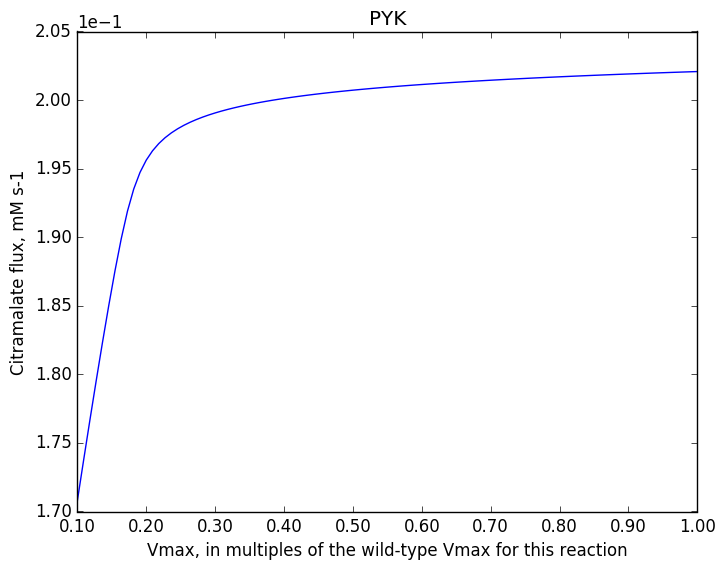
\includegraphics[scale=0.4]{issues_citraflux}
  \caption{Relationship between PYK $V_{max}$ and flux through citramalate synthesis reaction}
  \label{fig:issues_citraflux}

  \centering
  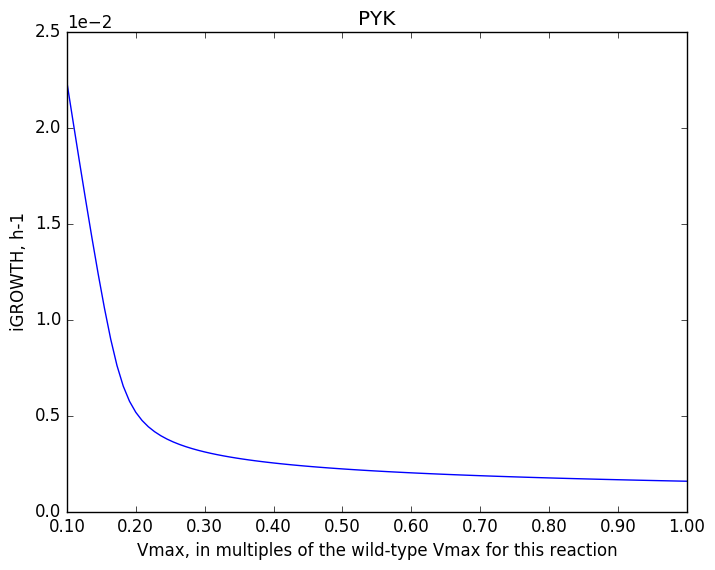
\includegraphics[scale=0.4]{issues_igrowth}
  \caption{Relationship between PYK $V_{max}$ and $\mathrm{iGROWTH}'$. iGROWTH is a species created to model growth in the kinetic model.}
  \label{fig:issues_igrowth}
\end{figure}

With this in mind, citramalate productivity can be used as the objective function instead of flux through citramalate synthesis in FBA. This would necessitate using libraries other than \texttt{cobra}, which is restricted to linear functions. CPLEX and Gurobi are potential alternatives, but do not suit a function that is not convex. Another alternative would be the use of flexible nets \citep{julvez_handling_2018}, which can also address uncertainties in the model.

%% SEPARATE SECTION??
% Species that break the steady-state threshold: comment on WHY I think they do
% ATP_MAINTENANCE/ATP_syn and BPG/OAA -- can these be ignored owing to the strange behaviour of the reactions? What roles do BPG and OAA play?
% GLCx and GLCp -- significant because glucose
% However it should be noted that the threshold was only broken when $V_{max}$ was at 0.1, a value unused later because it is in the `small' range that causes problems. Perhaps there is no need to worry about the species that break the threshold after all.

\subsection{Differential evolution}
\label{ssec:discussion-kinetic-de}

The results suggest that differential evolution is a useful genetic evolution algorithm to search for a combination of reaction $V_{max}$ values that maximises citramalate productivity. The maxima found in differential evolution agree with heatmaps, and seem to resolve complications that may be introduced by inflection points in the one-reaction plots. Importantly, using differential evolution predicted higher productivity than using one-reaction plots alone: using seven reactions from the one-reaction list, differential evolution predicted 1.56 times as much productivity compared to using the one-reaction plots.
Nevertheless, differential evolution has the `curse of dimensionality' as a limitation, and there are difficulties in finding optimal algorithm parameters for differential evolution.

The `curse of dimensionality' refers to the fact that, with an increasing number of dimensions, the difficulty of finding the optimal solution increases exponentially \citep{mier_small_2017}. The `curse' was reflected in the increased computation time and difficulty in reaching convergence when sets with more reactions were used. This was made worse by the memory leak in \texttt{roadrunner.RoadRunner()} and contributions from \texttt{libsbml.write-SBML\-To\-String()}, both of which had a large impact on the project as almost all scripts relied on them. Specifically, with \texttt{roadrunner}, memory could only be released when the Python program ended, and the model object must be passed into the simulation via a string intermediate instead of directly.

However, both optimisation of citramalate production and investigating glycolytic enzymes demonstrated that including few reactions could be sufficient. Specifically, with using glycolytic enzymes, adding reactions lower on the one-reaction list had little effect on citramalate productivity. The observation suggested that not all reactions in a network have to be included in differential evolution to produce valid results. This conclusion is beneficial as it reduces computation time needed to optimise citramalate productivity, and partially circumvents the memory leak described earlier.

Variants of differential evolution exist in the \texttt{scipy} and \texttt{pygmo} modules. These alternatives can use strategies other than \texttt{rand/1/bin} and can carry out self-optimisation of parameters. Furthermore, they can perform dithering on $F$, which was shown to improve convergence \citep{storn_usage_1996}. However, these alternatives took longer to compute and even exacerbated the memory leak problem, using up more memory for each iteration, presumably because they called the objective function more times. As they are black-box optimisation methods, I was unable to improve the algorithms.

% Other genetic algorithms? Why use differential evolution in particular? Please address this.

It remains to be seen how applicable the optimal $V_{max}$ values are to bacterial cultures. Optimal $V_{max}$ values for some reactions are at 0.1 $V_{max}$, at the lower boundary, and this may indicate that the activity of the corresponding enzyme should be minimised. Gene knockout studies preformed on the \emph{E. coli} MG1655 CimA3.7 mutant grown on XC growth medium suggest that the key knockout to optimise citramalate productivity is \emph{gltA} corresponding to citrate synthase \citep{wu_production_2016}. This agrees with the previous assertion; in support, GLT is second on the one-reaction list (after CITRA\_SYN) and consistently had its $V_{max}$ minimised in differential evolution. However, \citet{wu_production_2016} also suggest that \emph{ackA} (ACK/ACKr), \emph{acs} (ACS/ACS), \emph{pta} (PTA/PTAr), and \emph{poxB} are key reactions to be knocked out to optimise citramalate production, but these reactions are very low in the one-reaction list.
Additionally, there is the issue with translating optimal $V_{max}$ values to enzyme concentrations and appropriate gene expression control. 

%% SEPARATE SECTION?? ALSO NOT SURE IF IT EVEN SHOULD BE HERE AT ALL
% Investigating glucose uptake:
% The main text states that investigating glucose uptake was done to give insight between the intracellular and extracellular concentrations of glucose, and that this relationship is useful in determining the effects of a nutrient medium containing glucose on citramalate productivity. However, this was not really addressed in the Lund medium part of  the report.

% Information about decoupling between glucose exchange and glucose uptake relates to the relationship between the intracellular and extracellular concentrations of glucose. This relationship in turn would be useful in determining the effects of a nutrient medium containing glucose on citramalate productivity.


\section{Stoichiometric model}
\label{sec:discussion-stoichiometric}

\subsection{Relationship between the kinetic and stoichiometric models}
\label{ssec:discussion-stoichiometric-ks}

% Unit conversion (Jorge proposed a different number apart from 6.372)

% Boundaries for FBA:
The results suggest that kinetic model simulations are useful in informing the flux bounds for FBA on the stoichiometric model, and differential evolution is a useful strategy to establish such flux bounds. Specifically, the 41-dimension bounds found by differential evolution were mostly wider and bounds found by individually varying $V_{max}$ values in the kinetic model. However, it remains to be seen how realistic \emph{in vivo} are the highest and lowest possible flux values are.

Additionally, mapping reactions in the kinetic model to the stoichiometric model suggested a general strategy for mapping reactions that have one-to-one correspondence, and reconciling different sub-network structures for reactions that do not. Such a strategy may be applied to models of other metabolic networks.

\subsection{Flux balance analysis}
\label{ssec:discussion-stoichiometric-fba}

FBA suggested a fork between the growth and citramalate synthesis reactions, as evidenced by how optimising one excludes flux through the other. Alternatively, this phenomenon could be explained by how the fluxes of these reactions are not bounded, but this explanation is not realistic \emph{in vivo}. This observation may imply that optimising citramalate productivity in culture must take into account growth in addition to changing enzyme concentrations.

Analysis of the objective-exercise bounds covered flux ranges, reaction reversibility, and activity of reactions.
Having most flux bounds being near zero is expected for a large genome-scale metabolic model, suggesting regulation.
Investigating reversibility based on flux values correctly identified reactions established in the literature as irreversible. Nineteen reactions identified as reversible in the SBML model were only included in the 130 reactions deemed irreversible because they had a lower bound or an upper bound equal to zero.
Identifying reactions whose fluxes are forced to be non-zero identified ATP synthase as being constantly active, and identified 281 reactions with negative flux bounds, many of which are transport reactions. These observations are expected for self-maintenance of an \emph{E. coli} cell.
Thus, these findings confirm the validity of the 41-dimension flux bounds in the context of \emph{E. coli} \emph{in vivo}.

Finally, FVA and pFBA results are in agreement with that of FBA. Standard FVA may contain high absolute flux values that can only be high if they participate in loops, which are a mathematical artefact that cannot occur \emph{in vivo}. However, the FVA algorithm was unable to return results when the loopless condition in \texttt{cobra} was used. Ultimately, with my investigations, it may be sufficient to continue using FBA as it did not have such problems and took less computational time.

\subsection{Lund medium}
\label{ssec:discussion-stoichiometric-lund}

There are challenges to the validity of using a Monod model to relate $C_{glc}^{feed}$ to $C_{x}$ as in equation~\ref{eqn:taymaznikerel10_lreg}.  \citet{taymaz-nikerel_genome-derived_2010} suggest that there is a linear correlation betwen $D$ and $C_{x}$, with $r$ = 0.868, but for simplicity this factor was excluded as we only concern $D$ = 0.1.  With construction of the linear model, only three data points were used, but the lack of precision can be justified by our aim of finding a flux boundary rather than model the relations directly.  Additionally, \citet{kovarova-kovar_growth_1998} challenge Monod's model, but confirm that Monod's proposal and its slight modifications are sufficient to describe the growth of pure cultures with single growth-controlling sustrates under ideal conditions, supported by data for growth of \emph{E. coli} with glucose.

Through

\begin{equation}
  C_{x} = Y(C_{substrate}^{feed}  - C_{substrate}^{ext}),
\end{equation}
\label{eqn:monodmodel}

where $Y$ is the yield factor, the unit weight of cells formed per unit weight of substrate used \citep{schulze_relationship_1964}, it is implied that a linear regression model for $C_{x}$ with respect to $C_{glucose}^{feed}$ must have a negative vertical intercept, contrary to equation~\ref{eqn:taymaznikerel10_lreg}.  However, cell lysis may add a constant biomass concentration to the right-hand-side of~\vref{eqn:monodmodel} so that the intercept becomes positive.  \citet{taymaz-nikerel_genome-derived_2010} suggest that such cell lysis is significant.

Thus, I believe the methods were sufficient to determine an adequate lower limit for the rate of uptake of specific metabolites by the cell.

\section{Applications}
\label{sec:discussion-applications}

Translating findings from this project to \emph{in vivo} applications faces some challenges. Even if a combination of $V_{max}$ values that would optimise citramalate productivity can be found, obtaining such $V_{max}$ values \emph{in vivo} will have to take into consideration the biological variability in gene expression and may be hindered by poorly-characterised genes.

Additionally, this project demonstrated a strategy to use flux limits from the kinetic model and reaction mapping to enrich the stoichiometric model, improving on using FBA alone. Subsequently, FBA seemed useful in optimising productivity, especially with flux bound qualities agreeing with \emph{in vivo} qualities. Validity can be improved if citramalate productivity is used as the objective rather than flux through citramalate synthesis. However, this project has so far not been successful in extending this to study the effect of nutrient medium composition on metabolic models.

% \section{Future direction and suggestions}
% \label{sec:future}

% Improving or building up on this project may include some of the following:

% \begin{itemize}
% \item Use a simulator apart from \texttt{roadrunner} that does not have a memory leak
% \item Use standard deviations to quantify the effect varying $V_{max}$ values of each reaction in the kinetic model has on citramalate productivity
% \item Develop a method to investigate whether there are synergistic effects between reactions
% \item Investigate alternatives to \texttt{scipy} and \texttt{pygmo} for the implementation of a differential evolution algorithm, and investigating optimal parameter searches -- the fuzzy algorithm described by \citet{liu_fuzzy_2005} may be an option
% \item Use other genetic algorithms apart from differential evolution
% \item Use more than five iterations in differential evolution to generate bounds for FBA
% \item Investigate the theoretical basis behind mapping between the kinetic and stoichiometric models
%   \item Use CPLEX, Gurobi, or other packages to perform FBA using citramalate productivity as the objective function in place of flux through the citramalate synthesis reaction.
% \end{itemize}
  
% \section{Notes about files}
% \label{sec:files}

% The files included alongside this report include text files, images, spreadsheets, and Python scripts. The text files mainly contain information about the models, such as wild-type conditions, and results from various parts of the project. The images include the one-reaction plots and heatmaps. Important spreadsheets include an improved version of Anargyros's mapping spreadsheet and one to convert the minimum and maximum fluxes in the kinetic model to corresponding fluxes to be applied in FBA. Finally, the Python scripts were written to manipulate the two models, generate the images, and generate the data in the project. All files are version-controlled by Git.

\appendix
\chapter*{Appendix}
\addcontentsline{toc}{chapter}{Appendix}
\renewcommand{\thesection}{\Alph{section}}

The project took place at the Cambridge Systems Biology Centre, Department of Biochemistry, in Prof Steve Oliver's group. Research associate Dr Jorge J\'ulvez supervised me throughout the project. The project was entirely computational, and ran for eight weeks from 25 June 2018 to 17 August 2018.

Further work was done from 27 August 2018 to 3 October 2018, and resumed from 12 July 2019.

\section{Reactions in the kinetic model}
\label{ap:kineticreactionlist}

This is a list of the 68 reactions in the kinetic model with their wild-type $V_{max}$ values as specified in the SBML file. 49 reactions have $V_{max}$ as a parameter.

\begin{small}
\begin{longtable}{cS}
  \toprule
  Reaction & \multicolumn{1}{c}{Wild-type $V_{max}$ (mM s\textsuperscript{-1})}\\
  \midrule
  ACEA & 1.52595\\
ACEB & 0.352769\\
ACEK\_1 & \multicolumn{1}{c}{None}\\
ACEK\_2 & \multicolumn{1}{c}{None}\\
ACK & 7.23\\
ACN\_1 & 9.72413\\
ACN\_2 & 9.86571\\
ACS & 7.3\\
ADK & \multicolumn{1}{c}{None}\\
ATP\_MAINTENANCE & 1.30166\\
ATP\_syn & 108.733\\
CYA & \multicolumn{1}{c}{None}\\
CYTBO & 8.54045\\
DOS & \multicolumn{1}{c}{None}\\
EDA & 0.0775241\\
EDD & 0.111359\\
ENO & 11.7189\\
F6P\_E4P\_TKT & \multicolumn{1}{c}{None}\\
F6P\_GAP\_TAL & \multicolumn{1}{c}{None}\\
FBA & 21.6978\\
FBP & 0.215583\\
FUMA & 53.3414\\
GDH & 8.66573\\
GL6P\_HYDROLYSIS & \multicolumn{1}{c}{None}\\
GLC\_feed & \multicolumn{1}{c}{None}\\
GLT & 57.0584\\
GND & 4.08105\\
GPM & 10.9934\\
GROWTH & 9.74137\\
ICD & \multicolumn{1}{c}{None}\\
LPD & 0.0684413\\
MAD & 6.64269\\
MDH & 6.11492\\
MQO & 4.62283\\
NADH\_req & 23.0735\\
NDHII & 30.8306\\
PCK & 8.08777\\
PDH & 961.706\\
PFK & 0.185253\\
PGI & 2.32456\\
PGK & 16.1089\\
PGL & 11.5967\\
PIT & 7.146\\
PNT\_req & \multicolumn{1}{c}{None}\\
PPC & 21.439\\
PPS & 0.0163772\\
PTA & 2.7\\
PTS\_0 & \multicolumn{1}{c}{None}\\
PTS\_1 & \multicolumn{1}{c}{None}\\
PTS\_2 & \multicolumn{1}{c}{None}\\
PTS\_3 & \multicolumn{1}{c}{None}\\
PTS\_4 & \multicolumn{1}{c}{None}\\
PYK & 0.74716\\
RPE & 6.00103\\
RPI & 8.0\\
S7P\_E4P\_TAL & \multicolumn{1}{c}{None}\\
S7P\_R5P\_TKT & \multicolumn{1}{c}{None}\\
SDH & 1.56184\\
SK & 76.8163\\
SQR & 3.41617\\
TPI & 24.1843\\
X5P\_GAP\_TKT & \multicolumn{1}{c}{None}\\
XCH\_ACE1 & 100.0\\
XCH\_ACE2 & 100.0\\
XCH\_GLC & 100.0\\
XCH\_P & 100.0\\
ZWF & 0.2658\\
\_ACE\_OUT & \multicolumn{1}{c}{None}\\
\bottomrule
\end{longtable}
\end{small}

Of these, 41 correspond to real enzymes in \emph{E. coli}: ACEA, ACEB, ACK, ACN\_1, ACN\_2, ACS, ATP\_syn, CITRA\_SYN, CYTBO, EDA, EDD, ENO, FBA, FBP, FUMA, GDH, GLT, GND, GPM, LPD, MAD, MDH, MQO, PCK, PDH, PFK, PGI, PGK, PGL, PIT, PPC, PPS, PTA, PYK, RPE, RPI, SDH, SK, SQR, TPI, and ZWF.

\section{One-reaction list}
\label{ap:onereactionlist}

Here is the list of kinetic model reactions ordered by effect on citramalate productivity, as quantified by the method described in section~\ref{sec:onereac}. This list is termed the `one-reaction list' in this report.

\begin{small}
\pgfplotstabletypeset[
begin table = \begin{longtable},
col sep = comma,
display columns/0/.style={string type},
every head row/.style = {
  before row = \toprule,
  after row = \midrule
},
precision = 3,
every last row/.style = {
after row = \bottomrule
},
end table = \end{longtable}
]{onereactionlist.csv}
\end{small}

\section{41-dimension bounds}
\label{ap:41dbounds}

Here are the 41-dimension bounds for the 57 reactions that the stoichiometric and kinetic models have in common.

\begin{small}
\pgfplotstabletypeset[
begin table = \begin{longtable},
col sep = comma,
display columns/0/.style={string type},
every head row/.style = {
  before row = \toprule,
  after row = \midrule
},
precision = 4,
every last row/.style = {
after row = \bottomrule
},
end table = \end{longtable}
]{41dBoundaries-ori.csv}
\end{small}

\section{Mapping between the kinetic and stoichiometric models}
\label{ap:mapping}

Here is the mapping table to map reactions in the kinetic model to the stoichiometric model.

\begin{small}
  \pgfplotstabletypeset[
  column type =,
begin table = {\begin{tabularx}{\linewidth}{LLL}},
col sep = comma,
display columns/0/.style={string type},
display columns/1/.style={string type},
display columns/2/.style={string type},
display columns/3/.style={string type},
display columns/4/.style={string type},
every head row/.style = {
  before row = \toprule,
  after row = \midrule
},
precision = 4,
every last row/.style = {
after row = \bottomrule
},
end table = {\end{tabularx}}
]{mapping_condensed.csv}
\end{small}

%% NOTE TO SELF: DO NOT ATTEMPT TO INCLUDE THE OBJECTIVE-EXERCISE BOUNDS HERE BECAUSE THERE ARE 2,000 ENTRIES IN THE CSV FILE

% \section{Objective-exercise bounds}
% \label{ap:41dbounds}

% Here are the objective-exercise bounds. These bounds were obtained when I used the 41-dimension bounds to evaluate solutions for all reactions in the stoichiometric model in turn, both to maximise and to minimise flux through each reaction. The optimal minimum and optimal maximum values for each reaction formed the bounds shown here.

% \pgfplotstabletypeset[
% begin table = \begin{longtable},
% col sep = comma,
% display columns/0/.style={string type},
% every head row/.style = {
%   before row = \toprule,
%   after row = \midrule
% },
% precision = 4,
% every last row/.style = {
% after row = \bottomrule
% },
% end table = \end{longtable}
% ]{41dBoundaries-ori.csv}

% \section{Synergistic effects between reactions in the kinetic model}
% \label{ap:synergistic}

% I investigated whether there were synergistic effects between reactions by investigating reactions adjacent to each other, starting from the glycolytic pathway. No effects were observed for PGI and PFK, and a slight synergistic effect was observed for GPM and ENO. Between FBA and GDH, FBA exerts too little effect for the results to be conclusive. In contrast, ACEA and ACEB exhibit \emph{antagonistic} effects, and LPD and GDH, a pair of enzymes far apart from each other in the network seem to have a synergistic effect. Whether there were synergistic effects between reactions remains inconclusive. My investigations are in \texttt{kinetic/result/couples/Adjacent/Adjacent.txt}.

\printbibliography

\end{document}
